\documentclass[12pt, a4paper, openany]{book}
\usepackage[inline]{enumitem}
\usepackage{../generalStyle}
\usepackage{amsmath}

\begin{document}

\title{Basi di Dati - Appunti lezioni}
\author{
	Sara Angeretti\\
	\small{\href{https://t.me/Sara1798}{@Sara1798}}
}
\date{2022/2023}
\maketitle

\tableofcontents

\chapter{Introduzione al corso}
Turno T1 - AL
\\Da cancellare, per Elia, turno T1 AL ma ammettono anche MZ alle lezioni. L'importante è che gli AL sostengono l'esame con il prof di AL e gli MZ con il prof di MZ.
\section{I professori}
\begin{itemize}
    \item prof. Napoletano, di teoria (aula 1014 in U14).
    \\Per eventuali comunicazioni, mail: paolo.napoletano@unimib.it, ma \textbf{tassativamente} bisogna aggiungere la sigla [DB].
    \item prof.ssa Damiani, di esercitazione.
    \item prof. Raganato, di laboratorio.
\end{itemize}

\section{Organizzazione del corso}
\begin{itemize}
    \item lezioni teoriche ed analisi di casi studio (32 ore, pari a quattro crediti) PN 
    \item esercitazioni ed analisi casi studio (20 ore, pari a due crediti). CD 
    \item Laboratorio / esercitazioni (20 ore, pari a crediti). AR
\end{itemize}

\section{Organizzazione degli orari}
\begin{itemize}
    \item mercoledì: comincia a 10:30 spaccate
    \item giovedì: da definire perché c'è una lezione prima (statistica)
    \item venerdì lez: non ho capito io, ma per ora non li fa (marzo)
    \item venerdì lab: boh lo diranno.
\end{itemize}

\section{Organizzazione degli esami}
\subsection{Esoneri}
\begin{itemize}
    \item Ci sono parziali, circa seconda metà di aprile (\textbf{due} es di progettazione concettuale e modello relazionale) e seconda metà di giugno (\textbf{tre} es di SQL, algebra relazionale, progettazione logica).
    \item Per ora, i parziali sono aperti a tutti, ma il prof Napoletano deve sentire il prof Schettini del turno MZ.
\end{itemize}

\subsection{Totale}
\begin{itemize}
    \item Tutto il programma (quindi \textbf{cinque} es) è previsto per l'esame complessivo.
\end{itemize}

\subsection{Laboratorio}
\begin{itemize}
    \item A frequenza facoltativa ma essenziale, prevede una prova unica (sempre facoltativa) alla fine del laboratorio che permettere di avere un punteggio $-1 \leq p \leq 3$ da aggiungere alla media dei parziali o al voto del totale.
    \item Si lavorerà su MySQL, e prevede la progettazione concettuale e logica di una base di dati assegnata utilizzando lo strumento di Data Modeling fornito da MySQL.
    \item Il voto del laboratorio rimane valido tutto l'anno accademico, ovvero fino a Febbraio 2024 compreso, e andrà sempre sommato al voto preso.
\end{itemize}

\subsection{Valutazione}
\begin{itemize}
    \item Per superare l'esame, il voto minimo \textit{per parziale} è di \textbf{15/30}.
    \item Per superare l'esame, la \textit{media dei parziali} deve essere di \textbf{18/30}.
    \item Verrà eventualmente sommato il voto del laboratorio (se sostenuto).
\end{itemize}

\section{Il corso}
Le lezioni non verranno registrate, ma sono disponibili quelle dell'anno precedente.

\subsection{Il programma}
\begin{enumerate}
    \item Introduzione $\rightarrow$ prof. Napoletano
    \item Metodologie e modelli per il progetto delle basi di dati $\rightarrow$ prof. Napoletano
    \item La progettazione concettuale $\rightarrow$ prof. Napoletano
    \item Il modello relazionale \textbf{\textit{(pausa compitini)}} $\rightarrow$ prof. Napoletano
    \item SQL $\rightarrow$ prof.ssa Damiani
    \item Algebra relazionale $\rightarrow$ prof.ssa Damiani
    \item La progettazione logica $\rightarrow$ prof. Napoletano
\end{enumerate}
L'ordine degli argomenti è diverso da quello suggerito dal libro.

\subsection{Cosa vedremo}
Il corso e' dedicato a capire come e' organizzata una base di dati, a cosa serve, come si progetta, come si interroga e si crea.
% tre immagini da inserire

\chapter{Basi di Dati}
Una cosa che impareremo sarà \textbf{organizzare} il lavoro che ci viene presentato, per esempio da un eventuale cliente. Per prima cosa ci servirà un \textit{foglio dei requisiti}, ciò che dobbiamo progettare e sviluppare. Poi dovremo tradurre il passaggio da input ad output in una schematizzazione o mappa.

\section{Introduzione e definizioni}
\subsection{Risorse}
Le risorse di una azienda (o ente, amministrazione):
\begin{itemize}
    \item persone
    \item denaro 
    \item materiali 
    \item informazioni
\end{itemize}

\subsection{Basi di Dati}
Insieme organizzato di dati utilizzati per il supporto allo svolgimento di attività (di un ente, azienda, ufficio, persona).

\section{Sistemi informativi e sistemi informatici - una premessa}
Che cos'è l'informatica? Una definizione:
\begin{itemize}
    \item \textit{Scienza del trattamento razionale, specialmente per mezzo di macchine automatiche, dell'informazione, considerata come supporto alla conoscenza umana e alla comunicazione (Academie Francaise).}
    \item L'informatica ha due anime:
    \\- metodologica: i metodi per la soluzione di problemi e la gestione delle informazioni;
    \\- tecnologica: i calcolatori elettronici e i sistemi che li utilizzano; 
\end{itemize}
\begin{description}
    \item N.B.: \textbf{sistema informativo} $\neq$ \textbf{sistema informatico}
    \item[Sistema informativo] Componente (sottosistema) di una organizzazione che gestisce le informazioni di interesse (cioè utilizzate per il perseguimento degli scopi dell'organizzazione), le cui funzioni sono:
    \\ - acquisizione/memorizzazione
    \\ - aggiornamento
    \\ - interrogazione
    \\ - elaborazione
    \\N.B.: Il concetto di “sistema informativo” è indipendente da qualsiasi automatizzazione!! Anche prima di essere automatizzati, molti sistemi informativi si sono evoluti verso una razionalizzazione e standardizzazione delle procedure e dell'organizzazione delle informazioni.
    \item[Sistema informatico] Porzione automatizzata del sistema informativo: in pratica è la parte del sistema informativo che gestisce le informazioni con tecnologia informatica.
    % inserisci immagine sistemi_informatici_e_informativi1
\end{description}
Ma perché le basi di dati sono così importanti? Proviamo a definirle con degli aggettivi o caratteristiche che spieghino come mai sono così interessanti:
\begin{itemize}
    \item accessibili: le informazioni sono archiviate in modo ordinato;
    \item capienti: sono storate grandi quantità di dati;
    \item (facili da modificare;)
    \item ottimizzate: rapida ricerca delle informazioni; (comune a più sistemi)
    \item possibilità di raggruppare/filtrare le informazioni e schematizzarle/modellizzarle;
    \item sicurezza dei dati:;
    \item facilità di relazione dei dati;
    \item interfaccia per visualizzare in diversi modi;
    \item personalizzabili;
    \item scalabilità (Elia questa me la spieghi);
    \item interoperabilità: lavorabile con più linguaggi e strumenti;
    \item accesso concorrente alle informazioni: più persone possono lavorare allo stesso database o alla stessa sottosezione senza andare incontro ad inconsistenza dei dati;
    \item facilità di gestione delle ridondanze, che aiuta a ridurre al minimo l'inconsistenza dei dati;
    \item limitazione dell'inconsistenza dei dati: devono sempre essere consistenti, ovvero accessibili solo a chi ha diritto di farlo, il ruolo giusto;
\end{itemize}
Ma perché non usare una cosa più semplice come un FileSystem invece di un Database? Il primo mi aiuta con un'organizzazione logica, ma i Database sono dotati  di strumenti (tipo la progettazione modulare) che sono più efficienti.

\subsection{Sistema Informatico}
Gestisce un sistema informativo in modo automatizzato.
\\Garantisce che i dati siano conservati in modo permanente sui dispositivi di memorizzazione.
\\Permette un rapido aggiornamento dei dati per riflettere rapidamente le loro variazioni.
\\Rende i dati accessibili alle interrogazioni degli utenti.
\\Può essere distribuito sul territorio.

\section{Gestione delle informazioni}
Parole chiave:
\begin{itemize}
    \item Raccolta, acquisizione
    \item Archiviazione, conservazione
    \item Elaborazione, trasformazione, produzione
    \item Distribuzione, comunicazione, scambio
\end{itemize}

Nelle attività umane, le informazioni vengono gestite (registrate e scambiate) in forme diverse:
\begin{itemize}
    \item idee informali
    \item linguaggio naturale (scritto o parlato, formale o colloquiale, in una lingua o in un'altra)
    \item disegni, grafici, schemi
    \item numeri e codici
\end{itemize}
e su vari supporti
\begin{itemize}
    \item memoria umana, carta, dispositivi elettronici
\end{itemize}
Nelle attività standardizzate dei sistemi informativi complessi, sono state introdotte col tempo forme di organizzazione e codifica delle informazioni via via più precise (e in un certo senso artificiali).

\section{Informazioni e dati}
\textbf{Informazioni} $\neq$ \textbf{Dati}
\\Nei sistemi informatici (e non solo), le informazioni vengono rappresentate in modo essenziale, spartano: \textbf{attraverso i dati}.
\begin{itemize}
    \item \textbf{informazione}: notizia, dato o elemento che consente di avere conoscenza più o meno esatta di fatti, situazioni, modi di essere.
    \item \textbf{dato}: ciò che è immediatamente presente alla conoscenza, prima di ogni elaborazione; (in informatica) elementi di informazione costituiti da simboli che debbono essere elaborati. 
    \\I dati hanno bisogno di essere interpretati.
\end{itemize}
\textit{Esempio}:
\\'Mario' e '275' su un foglio di carta sono due dati. 
\\Se il foglio di carta viene fornito in risposta alla domanda “A chi mi devo rivolgere per il problema X; qual è il suo numero di telefono?”, allora i dati possono essere interpretati per fornire informazione e arricchire la conoscenza.
\\
\\\textbf{Ma perché i dati?}
\\La rappresentazione precisa di forme più ricche di informazione e conoscenza è difficile.
\\I dati costituiscono spesso una risorsa strategica, perché più stabili nel tempo di altre componenti (processi, tecnologie, ruoli umani)
\\I dati rimangono gli stessi nella \textit{migrazione} da un sistema al successivo.

\section{Basi di Dati}
\begin{description}
    \item[DB:] \textbf{Data Base} Collezione di dati utilizzati per rappresentare le informazioni di interesse di un sistema informativo.
    \item[DBMS:] \textbf{Data Base Management System}. Sistema software capace di gestire collezioni di dati che siano grandi, condivise e persistenti, assicurando la loro affidabilità e privatezza.
\end{description}
Accezione generica, \textbf{metodologica}: insieme organizzato di dati utilizzati per il supporto allo svolgimento delle attività di un ente (azienda, ufficio, persona).
\\Accezione specifica, \textbf{metodologica} e \textbf{tecnologica}: insieme di dati gestito da un DBMS.

\subsection{Altra definizione}
    Possiamo definire una BdD anche come: insieme di archivi in cui ogni dato e' rappresentato logicamente una sola volta e puo' essere utilizzato da un insieme di applicazioni da diversi utenti secondo opportuni criteri di riservatezza.

\subsection{caratteristiche}
\begin{itemize}
    \item i dati sono molti
    \item i dati hanno un formato definito
    \item i dati sono permanenti
    \item i dati sono raggruppati per insiemi omogenei di dati
    \item esistono relazioni specifiche tra gli insiemi di dati
    \item la ridondanza è minima e controllata: è assicurata la consistenza delle informazioni
    \item i dati sono disponibili per utenze diverse e concorrenti (anche contemporanee)
    \item i dati sono controllati: protetti da malfunzionamenti hardware e software 
    \item indipendenza dei dati dal programma    
\end{itemize}

\subsection{Perché studiare le basi di dati?}
Copia.

\subsection{Basi di dati multimediali}
Mi sono persa tutto.

\subsection{Data Base Management System - DBMS}
Un DBMS è un insieme di programmi che permettono di creare, usare e gestire una base di dati.
\\Quindi un DBMS è un sistema software general purpose che facilita il processo di definizione, costruzione e manipolazione del database per varie applicazioni.

\subsection{Creazione di un database}
\textbf{Tre fasi:}
\begin{itemize}
    \item definizione
    \item creazione/popolazione
    \item manipolazione
\end{itemize}

\subsection{Interrogazione di un database}
ziofrass
\begin{lstlisting}[mathescape=true]
    SELECT [Nome], [Cognome], [Indirizzo],
        [Citta]
    FROM Studenti
    WHERE [Cognome]="Rossi";
\end{lstlisting}

L'efficacia della query dipende da:
\begin{itemize}
    \item conoscenza del contenuto del db
    \item esperienza del linguaggio di interrogazione
\end{itemize}
oppure
\begin{itemize}
    \item semplicità ed efficacia dell'interfaccia di interrogazione
\end{itemize}

DataBase Management System
(DBMS)
• Sistema che gestisce collezioni di dati:
- grandi
- persistenti
- condivise
garantendo
- privatezza
- affidabilità
- efficienza
- efficacia

Hanno grandi dimensioni: dimensioni (molto) maggiori della memoria centrale dei sistemi di calcolo utilizzati; il limite deve essere solo quello fisico dei dispositivi.
Sono persistenti: hanno un tempo di vita indipendente dalle singole esecuzioni dei programmi che le utilizzano.
Sono condivise: ogni organizzazione (specie se grande) è divisa in settori o comunque svolge diverse attività; ciascun settore/attività ha un (sotto)sistema informativo (non necessariamente disgiunto).

\textbf{MI SONO PERSA UNA QUINDICINA DI SLIDES}

\section{Schemi e istanze}
In ogni base di dati esistono:
- lo schema, sostanzialmente invariante nel
tempo, che ne descrive la struttura, il
significato (aspetto intensionale).
• nell'esempio, le intestazioni delle tabelle
- l'istanza, i valori attuali, che possono
cambiare anche molto rapidamente (aspetto
estensionale)
• nell'esempio, il “corpo” di ciascuna tabella

lo schema costituisce l'aspetto intensionale,
ovvero la descrizione "astratta" delle
proprietà, ed è invariante nel tempo.
• L'istanza (i valori degli attributi) costituiscono
invece l'aspetto estensionale "concreto", che
varia nel tempo al variare della situazione di
ciò che stiamo descrivendo

Perso altre cinque SLIDES
ho rinunciato
ma cerca il sito DB engines rankings


\chapter{Argomento 2}


\chapter{Previsione I parziale}
\subsubsection{Quando}
Settimana 17-23 aprile.

\subsubsection{Argomenti}
\begin{description}
    \item[E-R:] abbiamo un testo in linguaggio naturale, dobbiamo creare uno schema concettuale con il linguaggio di modellazione E-R.
    \item[M-R:] abbiamo un piccolo testo, dobbiamo trovarne le chiavi primarie, i vincoli di integrità, i vincoli di dominio. 
\end{description}
Di solito è più facile il secondo esercizio, ma è importante fare bene il primo per poi fare il secondo.

\section{Modello dei dati relazionale}
Relazione -> teoria degli insiemi -> tramite sql
\\Due modelli:
\begin{itemize}
    \item modello a documenti (no-sql)
    \\si usa come strumento mongodb
    \item modello a serie temporali (time series)
\end{itemize}

\chapter{DBMS}
\section{Linguaggi per basi di dati}
Diversi tipi:
\begin{description}
    \item[L. per definizione dei dati:] Data Definition Languages - DDL
    \\ Si occupano della definizione degli schemi logici, fisici e delle autorizzazioni di accesso.
    \item[L. di manipolazione dei dati:] Data Manipulation Languages - DML
    \\Si occupano dell'interrogazione (\textbf{consultazione}) e aggiornamento (\textbf{manipolazione}) delle basi di dati.
\end{description}
Alcuni linguaggi come SQL (Structured Query Language) hanno funzioni di entrambe le categorie.

\subsection{Pagine web statiche/dinamiche}
Codice sorgente: linguaggio di \textit{scripting} (che usa dei \textit{tag}) HTML che è un linguaggio statico, che non permette dinamicità dei contenuti. Deve essere interpretato.
\\Sono nati altri linguaggi (tipo \textbf{php}, asp, jsp, etc...) che sono più \textit{dinamici} e riescono a replicare meglio le richieste dell'utente generando contenuti on-demand.
\\Quando una pagina dinamica deve mostrare i dati, accede ad una base di dati volta per volta per recuperare informazioni da mostrare.
\\Viene fatta una \textbf{query} per \textbf{accedere} ad una sezione ben definita di dati (es. informazioni di un utente sul sito Esse3 delle segreterie).
\\Posso fare una query anche per \textbf{manipolare} i dati (es. iscrizione ad un esame).

\section{Personaggi ed interpreti}
\begin{itemize}
    \item \textbf{progettisti} e realizzatori di \textbf{DBMS};
    \item \textbf{progettisti della base di dati} e amministratori della base di dati (DBA);
    \\Questi dovrebbero avere pieni poteri senza sforare nella "privatezza" dei dati.
    \\Def. dalle slides: Persona o gruppo di persone responsabile del controllo centralizzato e della gestione del sistema, delle prestazioni, dell'affidabilità, delle autorizzazioni. 
    \\Le funzioni del DBA includono quelle di progettazione, anche se in progetti complessi ci possono essere distinzioni.
    \item \textbf{progettisti} e programmatori \textbf{di applicazioni};
    \item \textbf{utenti}:
    \\- utenti finali (terminalisti): eseguono applicazioni predefinite (transazioni)
    \\- utenti casuali: eseguono operazioni non previste a priori, usando linguaggi interattivi
\end{itemize}

\section{Un esercizio per ripassare quanto detto}
\subsection{Es1}
Quali delle seguenti affermazioni sono vere?
\begin{itemize}
    \item l'indipendenza dei dati permette di scrivere programmi senza conoscere le strutture fisiche dei dati
    \\\textbf{VERO}
    \item l'indipendenza dei dati permette di modificare le strutture fisiche dei dati senza dover modificare i programmi che accedono alla base di dati
    \\\textbf{VERO}
    \item l'indipendenza dei dati permette di formulare interrogazioni senza conoscere le strutture fisiche
    \\\textbf{VERO}
\end{itemize}

\subsection{Es2}
Quali delle seguenti affermazioni sono vere?
\begin{itemize}
    \item il fatto che le basi di dati siano condivise
    permette di ridurre ridondanze e inconsistenze
    \item il fatto che le basi di dati siano persistenti ne
    garantisce l'affidabilità
    \\\textbf{VERO}
    \item il fatto che le basi di dati siano condivise rende
    necessaria la gestione della privatezza e delle
    autorizzazioni
    \\\textbf{VERO}
\end{itemize}

\subsection{Es3}
Quali delle seguenti affermazioni sono vere?
\begin{itemize}
    \item le istruzioni DML permettono di interrogare la base di dati ma non di modificarla
    \\\textbf{VERO}
    \item le istruzioni DDL permettono di specificare la struttura della base di dati ma non di modificarla
    \item 
    – non esistono linguaggi che includono sia istruzioni
    DDL sia istruzioni DML
    – SQL include istruzioni DML e DDL
    – le istruzioni DML permettono di interrogare la base
    di dati e di modificarla
    \\\textbf{VERO}
\end{itemize}

da sistemare
\\Gli esercizi che seguono sono utili per fissare i concetti, ma non ai fini dell'esercizio dell'esame.
\\
\\Cambia il pacco di slides.

\chapter{Progettazione di una base di dati}
Atzeni, Ceri, Paraboschi, Torlone, capitoli 6 e 7.
\\In questa parte del corso studieremo come
progettare una base di dati...
\\Verra’ illustrato ed esemplificato il processo di
progettazione concettuale e logica delle basi di dati
relazionali, che permette, partendo dai requisiti di
utente, di arrivare a produrre strutture di basi di dati di
buona qualità.
\\La progettazione di basi di dati è una delle attività
del processo di sviluppo dei sistemi informativi va
quindi inquadrata in un contesto più generale: il ciclo
di vita dei sistemi informativi

\section{Metodologie e modelli}
Un concetto importante di un'applicazione è \textbf{il ciclo di vita}.
\\\textbf{Def.:} insieme e sequenzializzazione delle attività svolte da analisti, progettisti, utenti, nello sviluppo e nell’uso dei sistemi informativi.
\\Attività iterativa, quindi “un ciclo”.
\begin{center}
    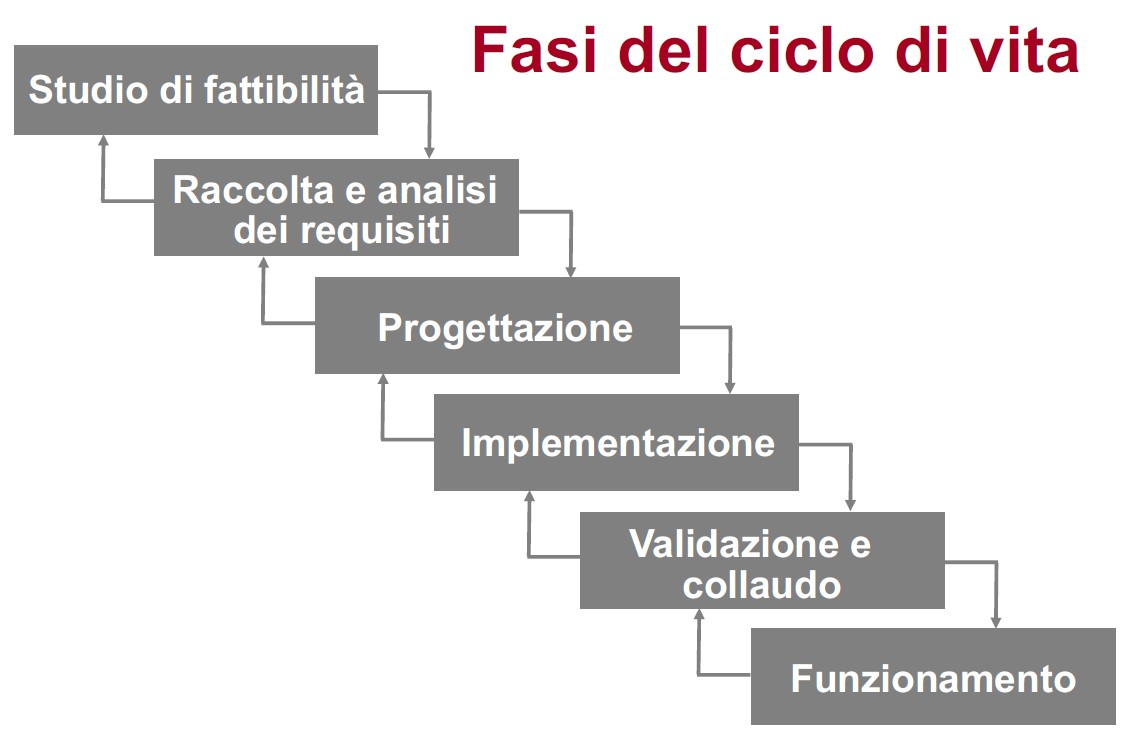
\includegraphics[width=0.75\textwidth]{chaptersLezioniSara/img/ciclo_di_vita1.jpg}
\end{center}
\begin{description}
    \item[Studio di fattibilità:] il progettista ha a che fare col committente (cliente) 
    \item[Raccolta e analisi dei requisiti:] viene prodotto un documento con i requisiti
    \item[Progettazione:] ER -> PL (?)
    \item[Implementazione:] si comincia
    \item[Validazione e collaudo:] di volta in volta, ci si confronta con l'utente o si controlla almeno di star seguendo i requisiti
    \item[Funzionamento:] non ho capito ma credo sia la fase finale, quindi la consegna del progetto finito. GUARDA LA SLIDE 8
\end{description}
Noi ci concentreremo sulla parte di progettazione, in particolare sulla modellizzazione dei dati.
\begin{center}
    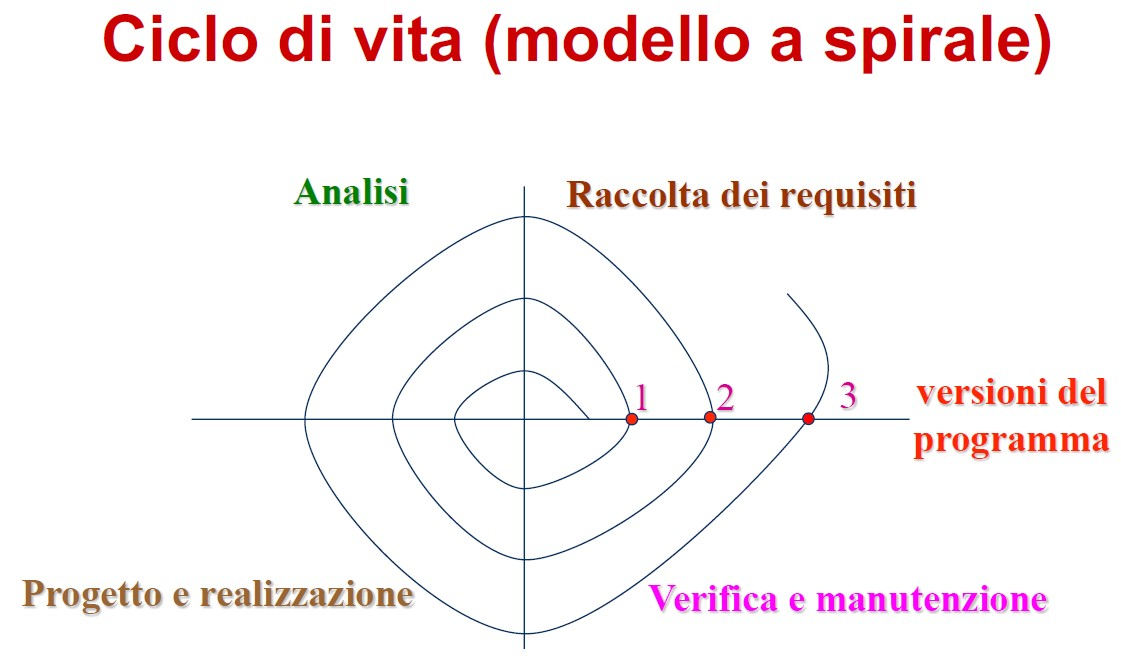
\includegraphics[width=0.75\textwidth]{chaptersLezioniSara/img/ciclo_di_vita2.jpg}
\end{center}
Ha balzato le slide di progettazione ma guardale.

\section{Progettazione}
Tre fasi:
\begin{center}
    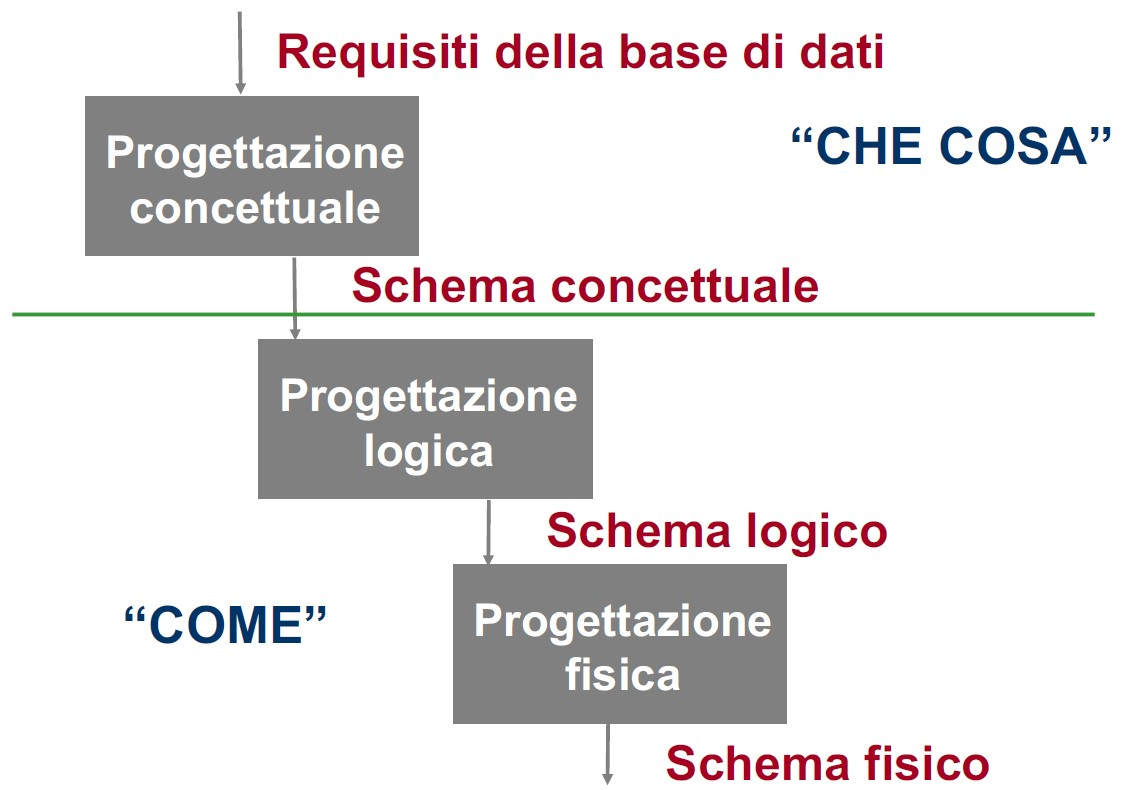
\includegraphics[width=0.75\textwidth]{chaptersLezioniSara/img/progettazione2.jpg}
\end{center}
A lezione vedremo p. concettuale e p. logica. La p. fisica sarà affrontata a laboratorio.
\begin{center}
    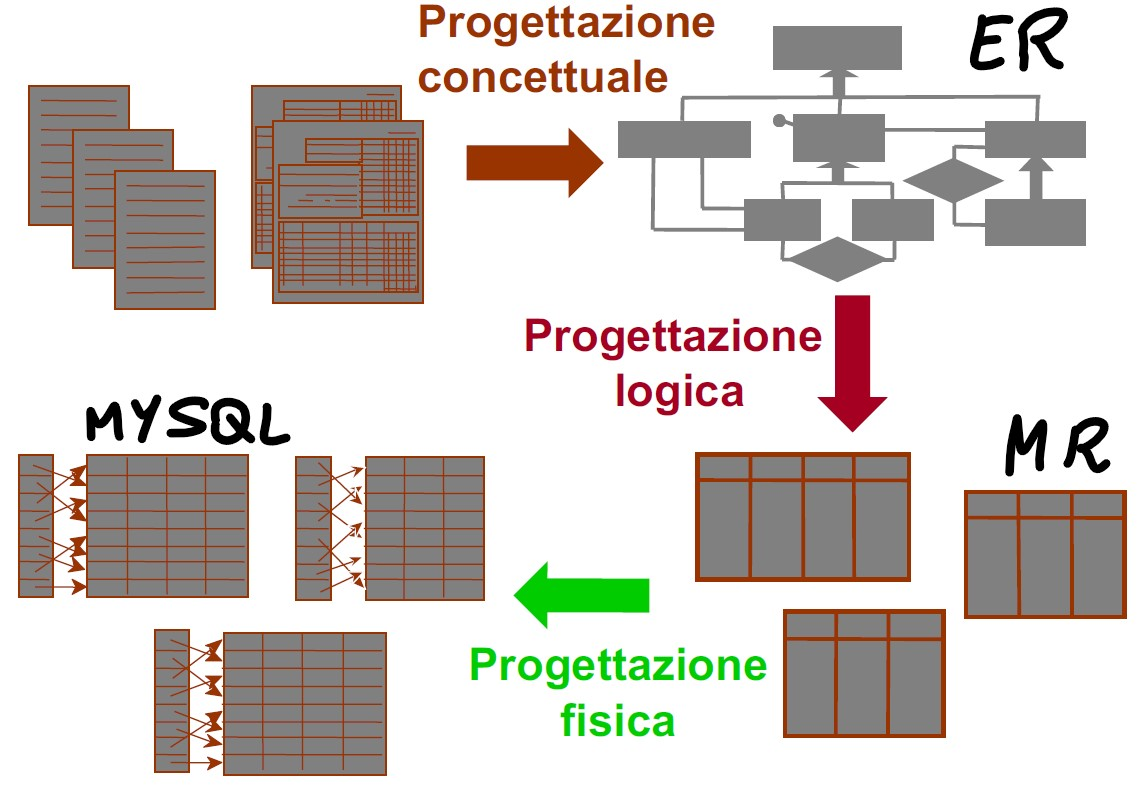
\includegraphics[width=0.75\textwidth]{chaptersLezioniSara/img/progettazione3.jpg}
\end{center}

\subsection{Fase di progettazione concettuale}
Progettazione concettuale: traduce i requisiti del sistema
informatico in una descrizione formalizzata, integrata delle
esigenze aziendali, espressa in modo indipendente dalle scelte
implementative (DBMS, SW e HW).
formale: la descrizione deve essere espressa con un
linguaggio non ambiguo e capace di descrivere in modo
soddisfacente il sistema analizzato;
integrata: la descrizione deve essere in grado di descrivere
nella globalità l'ambiente analizzato;
indipendente dall'ambiente tecnologico: la descrizione deve
concentrarsi sui dati e sulle loro relazioni, e non sulle scelte
implementative.

\subsection{Fase di progettazione logica}
La progettazione logica consiste nella traduzione dello
schema con concettuale nel modello dei dati del DBMS
Il risultato è uno schema logico, espresso nel DDL
del DBMS
In questa fase si considerano anche aspetti legati ai vincoli
ed all'efficienza
La progettazione logica si articola in due sotto-fasi:
•ristrutturazione dello schema concettuale
•traduzione verso il modello logico

\subsection{Fase di progettazione fisica}
Progettazione concettuale: traduce i
requisiti el sistema informatico in una descrizione
formale, integrata e indipendente dalle scelte
implementative (DBMS, SW e HW).
Progettazione logica: traduce lo schema
concettuale nel modello di rappresentazione
dei dati adattato dal DBMS scelto
Progettazione fisica: completa lo schema
logico ottenuto con le specifiche proprie
dell'hw/sw scelto. Il risultato e' lo schema
fisico che descrive le strutture di
memorizzazione ed accesso ai dati

\chapter{Introduzione al modello Entità-Relazione}
\section{Modello Entità-Relazione}
\begin{center}
    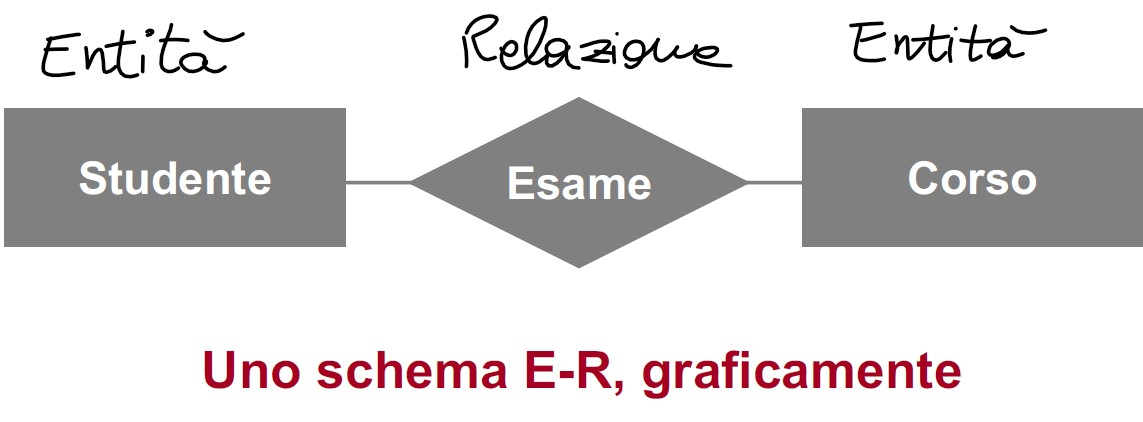
\includegraphics[width=0.75\textwidth]{chaptersLezioniSara/img/ER1.jpg}
\end{center}
Il modello ENTITÀ-RELAZIONE (E-R) è un
linguaggio grafico semi-formale per la
rappresentazione di schemi concettuali
•Il modello E-R si è ormai affermato come uno
standard nelle metodologie di progetto e nei sistemi
SW di ausilio alla progettazione
•Ne esistono molte versioni, (più o meno) diverse
l'una dall'altra.
•Entity-Relationship, P.P. Chen 1976

\`E una sottosezione di UML

\section{Entità}
\textbf{Def.:} Classe di oggetti (fatti, persone, cose) della applicazione di interesse con proprietà comuni e con esistenza “\textbf{autonoma}” e della quale si vogliono registrare fatti specifici.
\\\textit{Esempi:}
\begin{itemize}
    \item impiegato
    \item dipartimento
    \item città
    \item conto corrente
    \item università
    \item studente
\end{itemize}
L'essere autonoma di un'entità è un concetto fondamentale: es. gli studenti sono entità, gli esami sostenuti no perché non hanno un'esistenza autonoma.
\\\`E importante imparare, mentre stiamo leggendo un testo in linguaggio naturale, a capire chi può essere un'entità.
\subsection{Formalismi}
Si rappresentano con un rettangolo:
\begin{center}
    \includegraphics[width=0.75\textwidth]{chaptersLezioniSara/img/Entità1.jpg}
\end{center}
Ogni entità ha un nome che la identifica univocamente nello schema:
\begin{itemize}
    \item nomi espressivi
    \item opportune convenzioni (singolare)
\end{itemize}
A livello estensionale un'entità è costituita da un insieme di oggetti, che sono chiamati le sue istanze.
\\Ciò significa che, se in uno schema $S$ è definita una entità $E$, in ogni istanza $I$ dello schema $S$, alla entità $E$ è associato un insieme di oggetti (che viene denotato $istanze(I,\, E)) {e1, e2, e3, ..., e_n}$ (si chiama parte estensionale) che viene detto anche l'estensione di $E$ nella istanza $I$ dello schema $S$.
\\Una istanza di entità non è un valore che identifica un oggetto, ma è l'oggetto stesso.

\subsection{Occorrenza (o istanza) di entità}
\begin{itemize}
    \item 
•oggetto della classe che l'entità rappresenta
•Nello schema concettuale rappresentiamo le
entità, non le singole istanze (“astrazione”)
Quindi:
CONOSCENZA ASTRATTA -> entità
CONOSCENZA CONCRETA ->istanza di entità
\end{itemize}

\section{Attributi}
Un attributo di entità è una proprietà locale di un'entità,
di interesse ai fini dell'applicazione
• Un attributo associa ad ogni istanza di entità un valore
appartenente ad un insieme detto dominio dell'attributo
(tipicamente, interi, caratteri, stringhe, ecc.)
• Si definisce un attributo per l'entità E quando si vuole
rappresentare una proprietà locale delle istanze
dell'entità E.
Una proprietà di un oggetto si dice locale quando in
ogni istanza dello schema il valore di tale proprietà
dipende solamente dall'oggetto stesso, e non ha alcun
rapporto con altri elementi dell'istanza dello schema

\begin{center}
    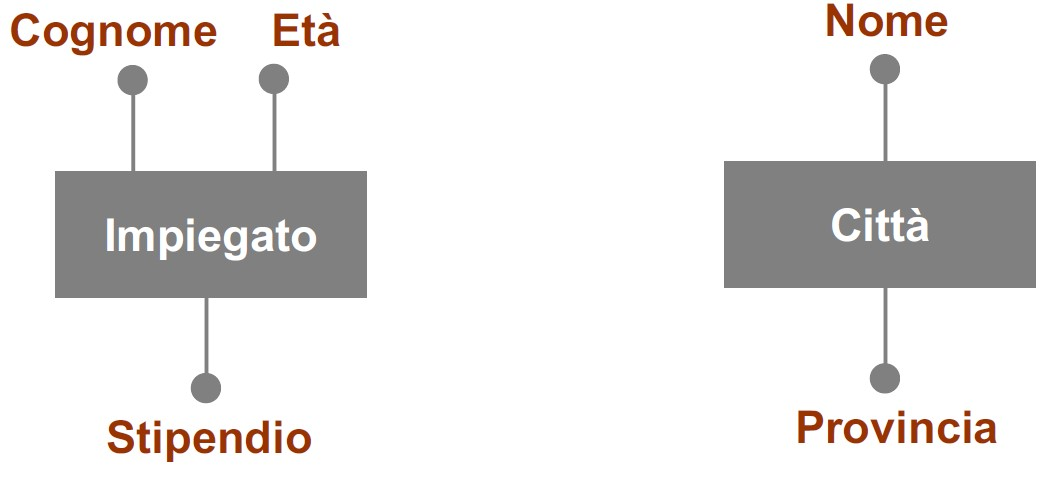
\includegraphics[width=0.75\textwidth]{chaptersLezioniSara/img/Attributi1.jpg}
\end{center}
Ogni attributo di entità ha un nome che lo identifica in modo
univoco nell'ambito della entità, ed è rappresentato da un
cerchio collegato alla entità a cui appartiene.

\begin{center}
    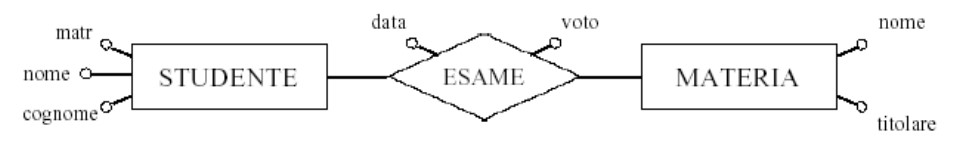
\includegraphics[width=0.75\textwidth]{chaptersLezioniSara/img/Attributi2.jpg}
\end{center}
Ogni attributo e' definito su un dominio di valori.
Un attributo associa ad ogni istanza di entità o associazione
un valore nel corrispondente dominio.
I domini solitamente non vengono specificati nell'E-R ma nella
documentazione associata. Se li si vuole indicare, la
notazione e' la seguente
\begin{center}
    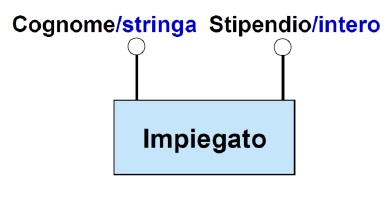
\includegraphics[width=0.75\textwidth]{chaptersLezioniSara/img/Attributi3.jpg}
\end{center}
Una entità può avere o no attributi.

\subsubsection{Attributi di entità}
\begin{center}
    \includegraphics[width=0.75\textwidth]{chaptersLezioniSara/img/Attributi_entità1.jpg}
\end{center}
Un'entità non può avere più di un valore per attributo. E non può averne neanche meno (oddio, veramente cambia in base al contesto, se ci fossero attributi facoltativi avrei dei \textbf{nulli}).
\\Gli attributi hanno un dominio, che ci specifica di che tipo di dati stiamo parlando.
\subsubsection{Attributi nulli}
I \textit{nulli} sono un concetto fondamentale nelle basi di dati.
\subsubsection{Attributi composti}
Si ottengono raggruppando attributi di una medesima entità o relazione che presentano affinità nel loro significato o uso.
\begin{center}
    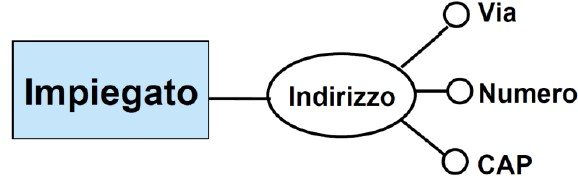
\includegraphics[width=0.75\textwidth]{chaptersLezioniSara/img/Attributi_composti.jpg}
\end{center}

\section{Relazione - Associazione}
Fatto che descrive un'azione o una situazione e che stabilisce legami logici tra istanze di entità (associa, mette in relazione) nella realtà che stiamo considerando.
\\I legami possono essere fra piu' di due entita'. Il numero di entità coinvolte in una relazione determina il suo grado (si vedano prossime slide).
\\NB: spesso useremo il termine ASSOCIAZIONE o RELATIONSHIP (per relazione) evitando confusione con la terminologia relazionale.
\subsection{Formalismi}
Si rappresentano con un rombo:
\begin{center}
    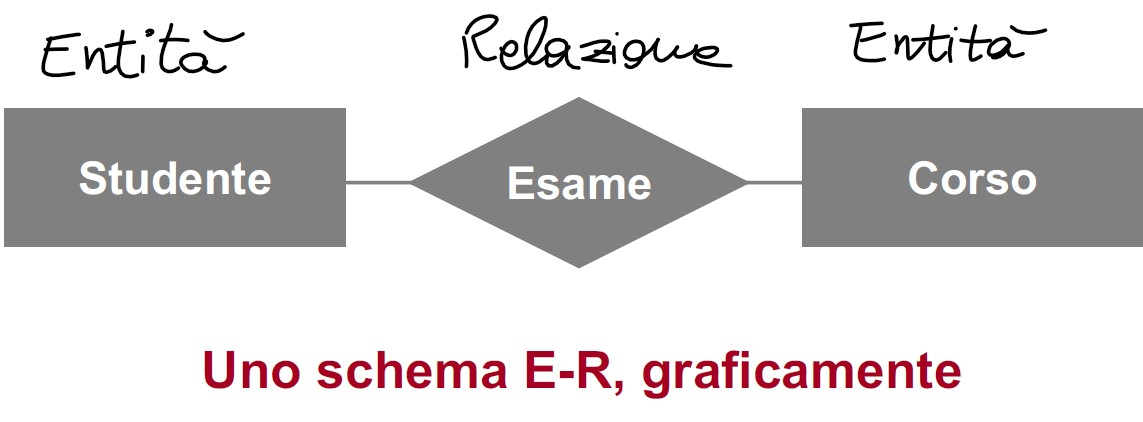
\includegraphics[width=0.75\textwidth]{chaptersLezioniSara/img/ER1.jpg}
\end{center}
Ogni relazione ha un nome che la identifica univocamente nello schema:
\begin{itemize}
    \item nomi espressivi
    \item opportune convenzioni (singolare, sostantivi invece che verbi)
\end{itemize}
A livello estensionale una relazione R tra le entità E ed F è
costituita da un insieme di coppie (x,y), tali che x è una istanza
di E, ed y è una istanza di F. Ogni coppia è detta istanza della
relazione R
• Ciò significa che, se in uno schema S è definita una relazione
R sulle entità E ed F, in ogni istanza I dello schema S, alla
relazione R è associato un insieme di coppie (denotato da
istanze(I,R)) {(x1, y1), (x2, y2), (x3, y3), …}
che viene detto anche l’estensione di R nella istanza I dello
schema S
• In altre parole, una relazione nel modello ER è, dal punto di
vista della semantica, una relazione matematica. In ogni
istanza I dello schema S si ha:
\begin{center}
    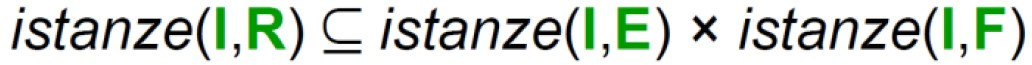
\includegraphics[width=0.75\textwidth]{chaptersLezioniSara/img/Relazioni1.jpg}
\end{center}

\subsection{Istanze di associazione}
\textbf{Def.:} combinazione (aggregazione) di istanze di entità che prendono parte alla associazione.
\\Es.:
•Rossi insegna Basi di dati
•Batini appartiene all’Università di Milano Bicocca
•La ditta Rossi ordina PC
•Bianchi lavora al magazzino 4
•Il tornio K22 è installato nell’officina 37
•il TIR 542 viaggia sulla tratta NA-MI

Es.:
\\Dalla semantica delle relazioni segue immediatamente che non possono esistere due istanze della stessa relazione che coinvolgono le stesse istanze di entità.
\begin{center}
    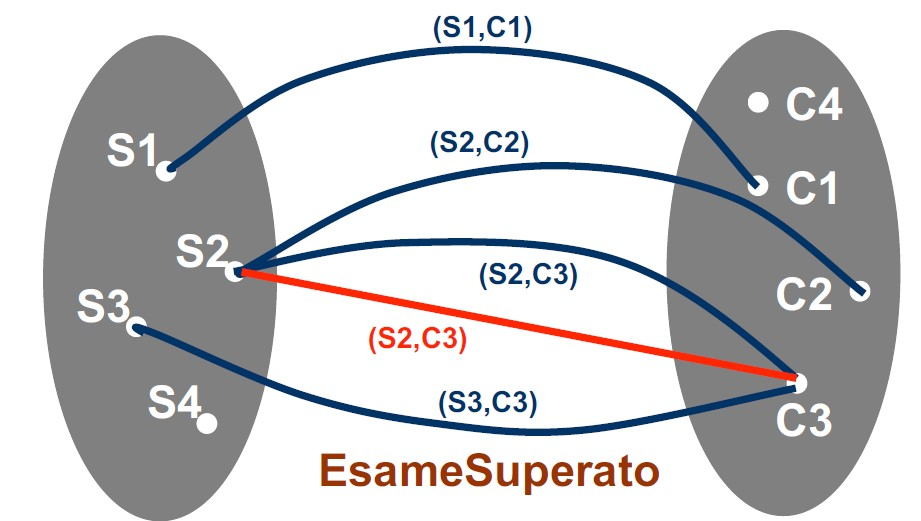
\includegraphics[width=0.75\textwidth]{chaptersLezioniSara/img/Relazioni2.jpg}
\end{center}
N.B.: due entità possono essere coinvolte in più relationship.
\begin{center}
    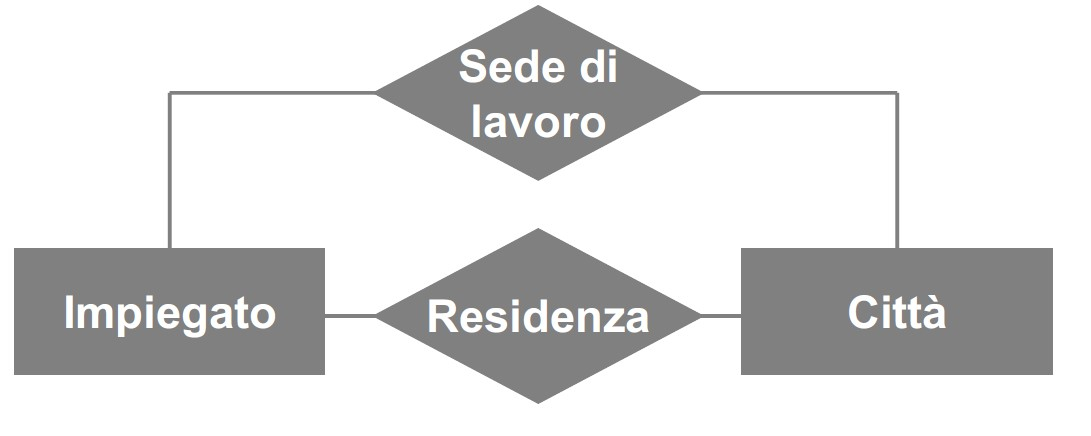
\includegraphics[width=0.75\textwidth]{chaptersLezioniSara/img/Relazioni3.jpg}
\end{center}
Le relationship possono coinvolgere più di due entità.
\begin{center}
    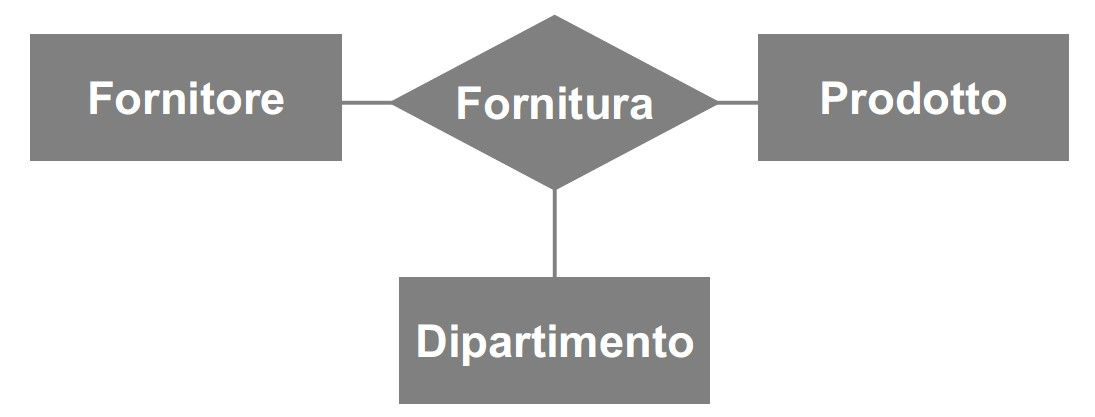
\includegraphics[width=0.75\textwidth]{chaptersLezioniSara/img/Relazioni4.jpg}
\end{center}

\subsubsection{Relazioni n-arie}
\begin{center}
    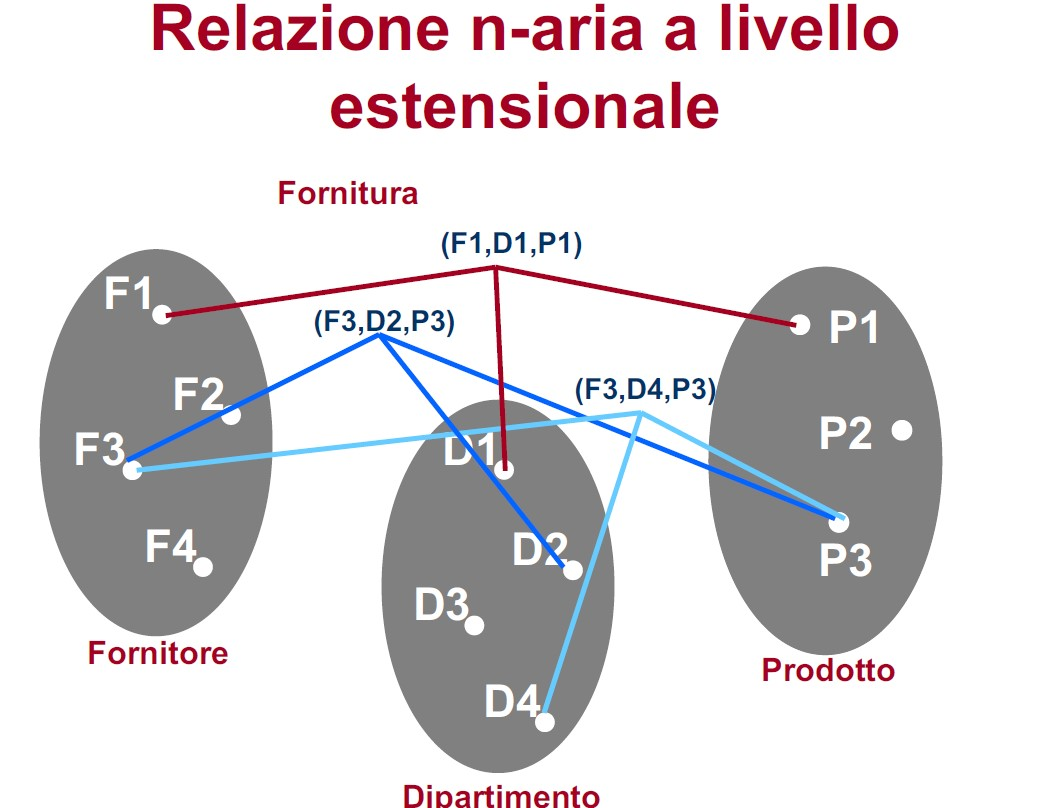
\includegraphics[width=0.75\textwidth]{chaptersLezioniSara/img/Relazioni5.jpg}
\end{center}
A livello estensionale (ovvero in ogni istanza I dello
schema S) una relazione R tra le entità E1,E2,…,En è
costituita da un insieme di n-ple (o tuple) (x1,x2,…,xn),
tali che x1 è una istanza di E1 in I, x2 è una istanza di
E2 in I,…, xn è una istanza di En in I. Ogni n-pla è detta
istanza della relazione R nella istanza I dello schema S
• Quindi, in ogni istanza I dello schema si ha:
\begin{center}
    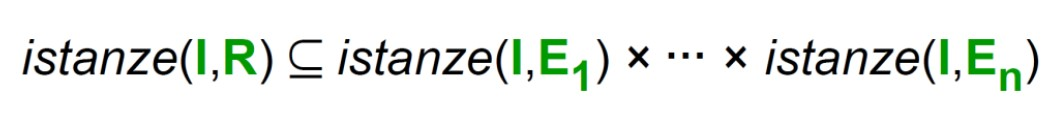
\includegraphics[width=0.75\textwidth]{chaptersLezioniSara/img/Relazioni6.jpg}
\end{center}

Una relazione può avere o no attributi.

\subsubsection{Attributi di relazione}
Un attributo di relazione è una proprietà locale di una
relazione, di interesse ai fini dell’applicazione
• Un attributo della relazione R tra le entita E1,E2,…,En
modella una proprietà non di E1, non di E2,…, non di
En, ma del legame tra E1,E2,…,En rappresentato da
R
• Un attributo associa ad ogni istanza di relazione un
valore appartenente ad un insieme detto dominio
dell’attributo

\subsubsection{Formalismi}
Ogni attributo di relazione ha un nome che lo identifica in
modo univoco nell’ambito della relazione, ed è
rappresentato da un cerchio collegato alla relazione a cui
appartiene.
\begin{center}
    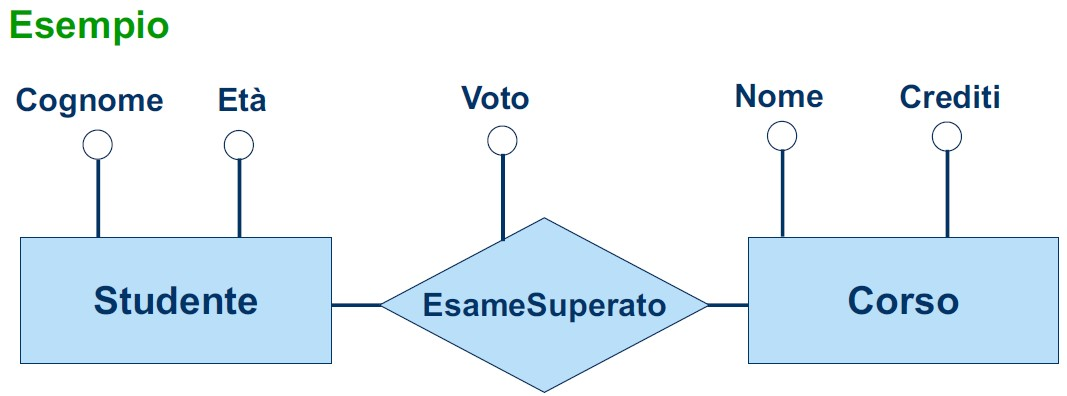
\includegraphics[width=0.75\textwidth]{chaptersLezioniSara/img/Attributi_relazione1.jpg}
\end{center}

Ho perso un po' di slides

\section{Entity-Relationship}


BLOB: Binary Long OBject. Sono i pallini pieni della rappresentazione degli attributi di entità.

cose

Es.
Descrivere lo schema concettuale della seguente realtà:
I docenti hanno un codice fiscale ed una età. I docenti operano nei corsi di laurea
(si dice che afferiscono ai corsi di laurea). Interessa la data di afferenza dei docenti
ai corsi di laurea. I corsi di laurea hanno un codice ed un nome, ed appartengono
alle facoltà. Ogni facoltà ha un nome.
\begin{center}
    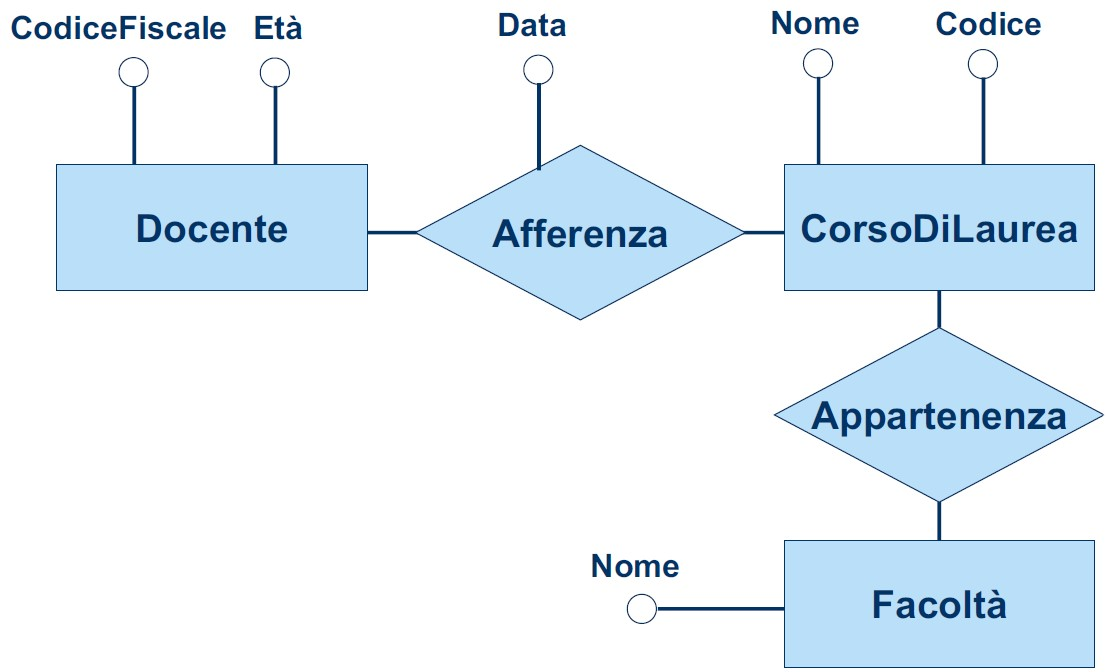
\includegraphics[width=0.75\textwidth]{chaptersLezioniSara/img/ER_es1_sol.jpg}
\end{center}

\subsection{Relazioni ricorsive}
Una associazione può coinvolgere “due o più volte” la stessa entità (associazione ricorsiva o ad anello). Questo ovviamente la fa classificare come relazione \textbf{binaria}, anche se c'è rappresentata una sola entità noi stiamo facendo una relazione tra due istanze di quell'entità, quindi conta come due.
\begin{center}
    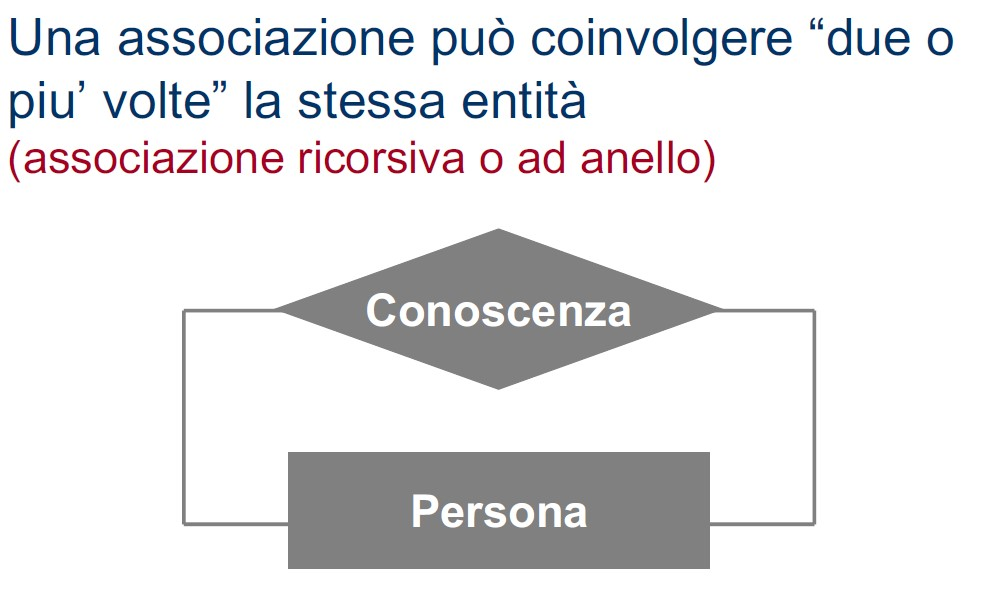
\includegraphics[width=0.75\textwidth]{chaptersLezioniSara/img/Relazioni_ricorsive1.jpg}
\end{center}
Ma siamo in grado da questo grafico di capire "chi viene prima e chi viene dopo"? No, se non operiamo sulla relazione: questo lo si fa aggiungendo dei "\textbf{ruoli}" alla relazione.
\begin{center}
    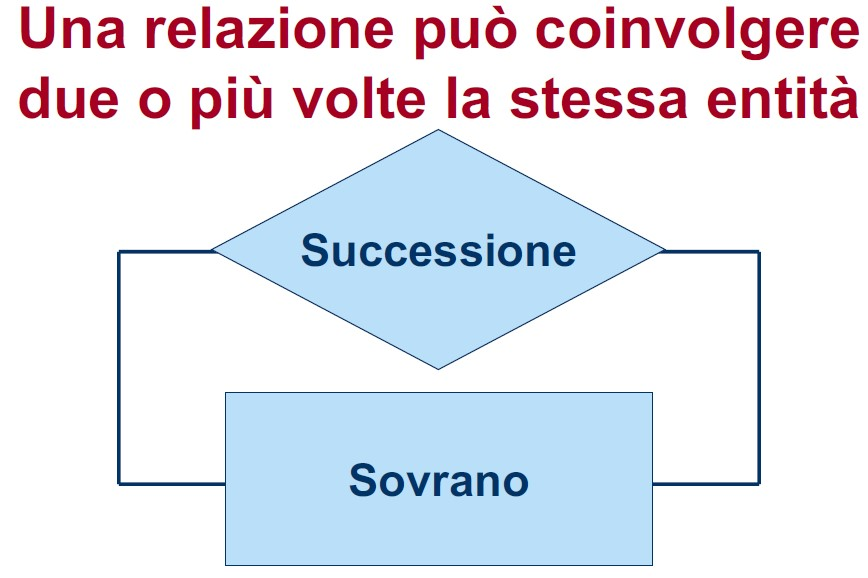
\includegraphics[width=0.75\textwidth]{chaptersLezioniSara/img/Relazioni_ricorsive2.jpg}
\end{center}
Problema: in una istanza di questo schema, data una coppia che è istanza di “Successione”, non si può individuare chi è il sovrano predecessore e chi il sovrano successore.
\subsubsection{I ruoli}
Nelle relazioni dove una stessa entità è coinvolta più volte è necessario aggiungere la specifica dei “ruoli”.

\subsubsection{Proprietà delle rel. ricorsive}
Un'associazione ad anello può essere o meno:
\begin{itemize}
    \item Simmetrica: $(a,\, b) \in A \Rightarrow (b,\, a) \in A$
    \item Riflessiva:$(a,\, a) \in A$
    \item Transitiva:$(a,\, b) \in A,  (b,\, c) \in A \Rightarrow (a,\, c) \in A$
    \item L'associazione conoscenza è simmetrica, irriflessiva e intransitiva.
\end{itemize}


vabbeh mancano slides

ultima cosa vista: esempio dei docenti uno migliore dell'altro
\section{Es.}
Oggi faremo degli esercizi, che faccio prima a mano e poi vedo se farli a pc o fare solo riferimento.
\\Convenzioni: entità - sostantivo singolare, relazione - verbo singolare.
\\Slide 82: corsivo entità, grassetto relazioni.
\\Descrivere lo schema concettuale della seguente realtà:
\\Degli \textit{impiegati} interessa il codice fiscale, il nome, il cognome, i dipartimenti ai quali \textbf{afferiscono} (con la data di afferenza), ed i \textit{progetti} ai quali \textbf{partecipano}. Dei progetti interessa il nome, il budget, e la città in cui \textbf{hanno luogo} le corrispondenti attività. Alcuni progetti sono parti di altri progetti, e sono detti loro \textbf{sottoprogetti}. Dei \textit{dipartimenti} interessa il nome, il numero di telefono, gli impiegati che li \textbf{dirigono}, e la \textit{città} dove è \textbf{localizzata} la sede. Delle città interessa il nome e la regione.
\\Entità:
\begin{itemize}
    \item impiegato
    \item progetto
    \item dipartimento
\end{itemize}
Relazioni:
\begin{itemize}
    \item afferire
    \item partecipare
    \item avere luogo
    \item fare parte/sottoprogetto (ruolo)
    \item dirigere
    \item essere localizzato
\end{itemize}

\subsubsection{Ma domanda: quando un attributo viene classificato come entità?}
Come faccio, leggendo un testo, a capire quando un elemento che mi sembra un attributo possa invece essere effettivamente scritto come entità?
\begin{enumerate}
    \item è descritto da più di un attributo
    \item partecipa a più di una relazione
    \item è autonoma
\end{enumerate}
C'è una slide.

\subsubsection{Come invece scegliere se entità o relazione?}
C'è una slide.

Torniamo alla teoria.
\section{Cardinalità di una relazione}
Si indica come $(x,\, y)$ dove $x$ è la cardinalità minima dell'associazione e $y$ è la cardinalità massima dell'associazione.
\\Si legge "Entità1 è in relazione con $x$ Entità2 o al più con $y$ Entità2".
\\Simboli standard:
\begin{itemize}
    \item $0$: cardinalità minima, indica partecipazione facoltativa;
    \item $1$: cardinalità minima, indica partecipazione obbligatoria;
    \item $n$: cardinalità massima.
\end{itemize}

\subsection{Classificazione delle relazioni}
Praticamente lo decide la cardinalità massima il nome.
\begin{itemize}
    \item uno a uno: $(1,\, 1) <-> (0,1)$
    \item va beh
    \item .
\end{itemize}

\subsection{Cardinalità degli attributi}
è possibile associare delle cardinalità anche agli attributi, per:
- indicare opzionalità
- indicare attributi multivalore




\section{Riassunto: Identificatori}
L'abbiamo vista la volta scorsa. Fa l'esempio dello studente e dell'università, in cui l'attributo Matricola di Studente è debole perché è sufficiente nel contesto di una sola università, dove è un identificativo univoco. Ma se consideriamo le università di tutt'Italia, non è più univoco.
\\Serve allora un identificatore esterno.
\subsubsection{Requisiti}
Avere una relazione 1 a molti, ovvero $(1,\, 1) --> (0,\, n)$.

\section{Ereditarietà}
\subsection{Relazione IS-A (o IS-A) tra entità}
Se avessi una entità studente, con attributi matricola (pallino pieno) che nel contesto di 1 università è univoca quindi sufficiente, nome e cognome.
\\Fra questi ho particolari istanze chiamate studenti-lavoratori che hanno come attributi inizio-lavoro e sede-lavoro. Questo sottoinsieme (chiamato anche "relazione is-a") si comporta come in programmazione 2. Ovvero:
\begin{itemize}
    \item studenti-lavoratori eredita tutti gli attributi di studenti
    \item non è vero il contrario
\end{itemize}
Ma avremmo potuto anche fare un solo attributo "sede di lavoro" per dire che se c'è, allora è uno studente-lavoratore per evitare tutto il sottoinsieme. Perché non l'abbiamo fatto?
\\Principalmente per facilità di rappresentazione e lettura del modello. Poi anche per specificare che gli attibuti del sottoinsieme sono esclusivi, specifici delle istanze di quel sottoinsieme e non di tutte le istanze di studente.
\\Tornando alle slides:
\begin{itemize}
    \item Fino ad ora non abbiamo detto nulla sul fatto se due
    entità possano o no avere istanze in comune
    \item \`E facile verificare che, in molti contesti, può accadere che tra due classi rappresentate da due entità nello schema concettuale sussista la relazione IS-A (o relazione di sottoinsieme), e cioè che ogni istanza di una sia anche istanza dell'altra. (Es. Studente, Studente della laurea breve)
    \item La relazione IS-A nel modello ER si può definire tra
    due entità, che si dicono “entità padre” ed “entità figlia” (o sottoentità, cioè quella che rappresenta un sottoinsieme della entità padre) (Es Studente è entità padre di Studente della laurea breve)
\end{itemize}
Poi ci sono 4-5 slides da sistemare sull'ereditarietà. Ovviamente NB che le relazioni che un eventuale sottoinsieme può avere con altre entità sarà specifica di quel sottoinsieme, così come per gli attributi vale anche per le relazioni.

\section{Generalizzazione tra entità}
Dalle slides:
\begin{itemize}
    \item Finora, abbiamo considerato la relazione ISA che stabilisce che l'entità padre è più generale della sottoentità. Talvolta, però, l'entità padre può generalizzare diverse sottoentità rispetto ad un unico criterio. In questo caso si parla di generalizzazione.
    \item Nella generalizzazione, le sottoentità hanno insiemi di istanze disgiunti a coppie (anche se in alcune varianti del modello ER, si può specificare se due sottoentità della stessa entità padre sono disgiunte o no).
    \item Una generalizzazione può essere di due tipi:
    \\• Completa (o totale): l'unione delle istanze delle sottoentità è uguale all'insieme delle istanze dell'entità padre. Si rappresenta con una freccia piena.
    \\• Non completa (o parziale). Si rappresenta con una freccia non piena.
\end{itemize}
Parliamo di generalizzazione \textbf{esclusiva} quando un'entità è composta da due sottoinsiemi che raggruppano le istanze e nessuna istanza sta fuori da questi due sottoinsiemi (si dice anche completa) e l'intersezione dà l'insieme vuoto. $$\cup_i E_i = E$$ $$\cap_i E_i = \emptyset$$
\\ ---
\\Se invece avessimo $$\cup_i E_i = E$$ $$\cap_i E_i = \emptyset$$

Abbiamo 4 casi:
\begin{itemize}
    \item completa, esclusiva
    \item completa, non esclusiva
    \item non completa, esclusiva
    \item non completa, non esclusiva
\end{itemize}

Come passo da non esclusiva a esclusiva? Andando a recuperare l'intersezione e rendendola entità a sé.

\section{esempio sessista e antico}
\begin{itemize}
    \item Le persone hanno CF, cognome ed età; gli uomini anche la posizione militare; 
    \item gli impiegati hanno lo stipendio e possono essere segretari, direttori o progettisti (un progettista può essere anche responsabile di progetto); 
    \item gli studenti (che non possono essere impiegati) un numero di matricola;
    \item esistono persone che non sono né impiegati né studenti (ma i dettagli non ci interessano)
\end{itemize}
Soluzione: slide successiva

\section{Altre proprietà}
possono esistere gerarchie a più livelli e multiple
generalizzazioni allo stesso livello
• un'entità può essere inclusa in più gerarchie, come
genitore e/o come figlia
• se una generalizzazione ha solo un’entità figlia si
parla di sottoinsieme

\section{Riassunto finale: tutto quello che abbiamo visto di ER}
Slide 157 in poi


Esercitazioni
175(immobili) tutto falso
176(città) tutto falso tranne le ultime due
\chapter{Progettazione concettuale}
Diverse fasi:
% img1
% img2
\section{Analisi dei dati}
Anche nota come "Analisi dei requisiti e progettazione concettuale".
\\Comprende attività (interconnesse) di
\begin{itemize}
    \item acquisizione dei requisiti
    \item analisi dei requisiti
    \item costruzione dello schema concettuale
    \item costruzione del glossario
\end{itemize}

\subsubsection{Requisiti}
Possibili fonti:
\begin{itemize}
    \item utenti, attraverso:
    \\• interviste
    \\• documentazione apposita
    \item documentazione esistente:
    \\• normative (leggi, regolamenti di settore)
    \\• regolamenti interni, procedure aziendali
    \\• realizzazioni preesistenti
    \item modulistica
\end{itemize}

\subsection{Acquisizione e analisi dei requisiti}
Il reperimento dei requisiti è un'attività difficile e non standardizzabile.
\\L'attività di analisi inizia con i primi requisiti raccolti e spesso indirizza verso altre acquisizioni.
% \\Ho perso tipo 75 slide

% tutto in subsubsection

\section{Scrittura dei requisiti}

\section{Strutturazione dei requisiti}

\section{Specifiche sulle operazioni}

\section{Dalle specifiche al modello ER}

\section{Design Pattern}
Soluzioni progettuali a problemi comuni. Sono largamente usati nell'ingegneria del software.
\\Vediamo alcuni pattern comuni nella progettazione concettuale di basi di dati.
\\Parliamo di \textbf{reificazione}: procedimento di creazione di un modello di dati basato su un concetto astratto predefinito.
\subsection{Reificazione}
% c'è una slide

\subsubsection{Part-of}
L'unicità è un tema importante: un identificativo unico mi identifica una sola istanza, non ci saranno altre istanze di quell'entità con quell'identificativo.
\\A volte un entità può essere legata a un'altra entità creando una relazione di tipo 1,N. Gli esempi mostrano come il concetto di part of possa essere di dipendenza (Sala non esiste senza Cinema) o meno (Tecnico è autonomo da Team).
\\NB: avevamo detto che l'identificatore esterno non è univoco sempre, ma ci serve una situazione univoca (es. della matricola dell'università, univoca in una università ma non tipo in tutta la Lombardia): perciò funziona solo in una relazione 1 a molti.
\\NBB: se la relazione è 1 a molti, l'entità che ha l'identificatore esterno è quella che ha la cardinalità 1. Grazie, copilot.
\\NBBB: la cardinalità della relazione si guarda col numerino a destra, ovvero la cardinalità massima. Diversi casi:
\begin{itemize}
    \item (*, 1) -> (*, n): 1 a molti
    \item (*, 1) -> (*, 1): 1 a 1
    \item (*, n) -> (*, 1): molti a 1
    \item (*, n) -> (*, n): molti a molti
\end{itemize}

\subsubsection{Istance-of}
\\A volte si viene a creare la necessità di creare un'entità astratta che prende concretezza in un'entità istanza. Volo possiede informazioni astratte sul Volo Reale che invece rappresenta il volo che avviene giornalmente. (vedi esempio grafico)

\subsubsection{Reificazione di relazione binaria}
Nell'esempio degli esami, la relazione diventa un'entità dove l'attributo debole "data" diventa un attributo esterno quando reso univoco tramite un legame con un attributo "matricola" dell'entità "studente", che è univoco (pallino pieno). Questo è rappresentato dal secondo modello. Nell'esempio, non potendo avere ripetizioni, non posso sostenere due volte nello stesso giorno lo stesso esame. Posso due esami diversi. Il secondo modello grafico mi andrebbe bene. Però posso farlo guardando il terzo modello grafico.

\subsubsection{Nota sull'identificazione esterna}
Non esistono due esami diversi che riguardano la stessa coppia di studente e corso.
% img
L'esempio mostra che un identificatore esterno può anche non comprendere attributi, e può coinvolgere una sola relazione attraverso un unico ruolo.
% tante slide che mi sono persa

\section{Strategie di progetto}
\chapter{Message-oriented communication}
\subsubsection{Cosa vedremo in questa sezione}
Message-oriented communication:
\begin{itemize}
    \item The Web and HTTP messages
    \item Messages communication vs stream communication
\end{itemize}
Communication types
\begin{itemize}
    \item Synchronous and asynchronous communication
    \item Persistent and volatile communication
    \item Queue-based communication
\end{itemize}

\section{L'architettura del Web}
Il Web supporta l'interazione tra client e server via HTTP.
\begin{center}
    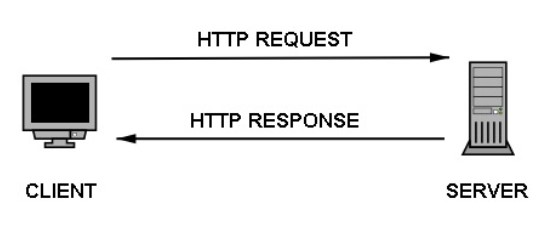
\includegraphics[width=0.675\textwidth]{img/MOC_architetture1.jpg}
\end{center}
Il client è realizzato da un “Browser” o “User-Agent”
\\Il server è realizzato da un “Web Server” o “HTTP Server”

\subsection{Il browser}
Il browser è l'applicazione per il Web sul lato del client.
\\Un web browser (detto User-Agent) è un programma che consente la navigazione nel Web da parte di un utente.
\\La funzione primaria di un browser è quella di interpretare il codice con cui sono espresse le informazioni (pagine web) e visualizzarlo (operazione di rendering) in forma di ipertesto.
\begin{itemize}
    \item I browser moderni hanno anche funzioni più avanzate per
    \\- trattare altri tipi di dati: es. Multimedialità, RSS, XML, JSON …
    \\- ospitare ed eseguire applicazioni: es. JavaScript (vedremo più avanti)
    \item Il rendering dipende dal dispositivi utilizzati, anche “non visuali”, ad esempio per supportare utenti non vedenti, es.:
    \\- sintesi vocale
    \\- alfabeto Braille
    \\...
\end{itemize}

\subsection{Web Page}
Una pagina web (web page, o anche documento) è costituita da diversi oggetti (risorse nella terminologia del web).
\\Una risorsa è un file, cioè una sequenza di dati (in formato digitale) residente in un computer, che è identificato da una URL (cioè un indirizzo univoco per la risorsa).
\begin{itemize}
    \item Testo, immagini, musica, …
\end{itemize}
La maggior parte delle pagine web sono costituite da un file HTML che definisce la struttura e i contenuti della pagina, testuali più altri oggetti.
\begin{itemize}
    \item HTML: HyperText Markup Language, è il linguaggio con cui si scrivono gli ipertesti (si definisce la struttura di una pagina, i collegamenti, si inseriscono immagini, …)
\end{itemize}
Un Web Server è una applicazione che si occupa di gestire le risorse (file) su un computer e di renderle disponibili ai client.

\subsection{Gli ipertesti}
Un ipertesto (hypertext) è un insieme di testi o pagine leggibili con l'ausilio di un'interfaccia elettronica, in maniera non sequenziale, tramite hyperlink (o più semplicemente link, cioè collegamenti), che costituiscono un rete raggiata o variamente incrociata di informazioni organizzate secondo criteri paritetici o gerarchici (es. menu).
\begin{center}
    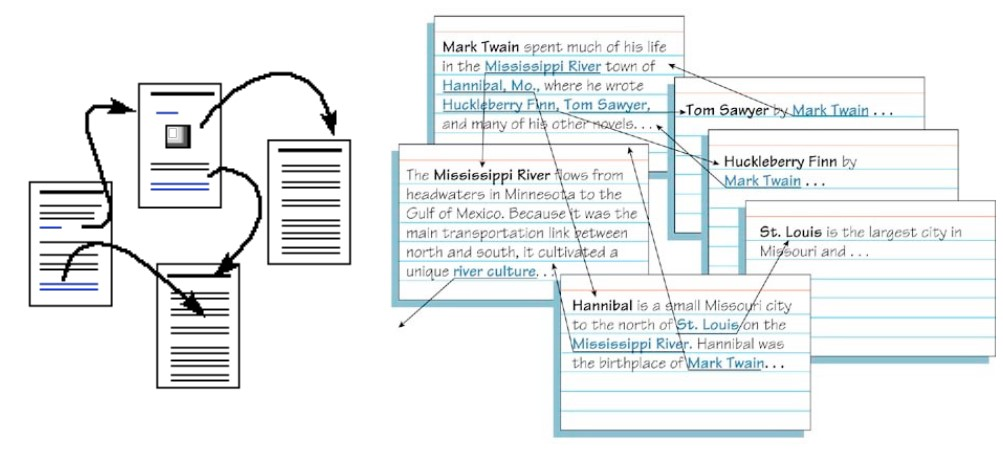
\includegraphics[width=0.675\textwidth]{img/MOC_architetture2.jpg}
\end{center}

\subsection{URL(Uniform Resource Locator)}
Identifica un oggetto nella rete e specifica come interpretare i dati ricevuti attraverso il protocollo.
\\Ha cinque componenti principali:
\begin{enumerate}
    \item nome del protocollo
    \item indirizzo dell'host
    \item porta del processo (la controparte)
    \item percorso nell'host
    \item Identificatore della risorsa
\end{enumerate}
\begin{verbatim}
    protocollo://indirizzo_IP[:porta]/cammino/risorsa
          1.          2.         3.      4.      5.
    ftp://www.adobe.com/dawnload/acroread.exe
    http://www.biblio.unimib.it/go/Home/Home-English/Services
    http://www.biblio.unimib.it/link/page.jsp?id=47502837
    http://www.someSchool.edu/someDept/pic.gif
    http://www.someSchool.edu:80/someDept/pic.gif
\end{verbatim}

\subsection{I linguaggi del Web}
I dati testuali sono espressi in linguaggi standard:
\begin{itemize}
    \item HTML (per definire la struttura dei contenuti e la loro impaginazione)
    \item può contenere CSS (per gestire la presentazione, cioè il rendering), …
    \item XML (focalizzato sui dati e la loro struttura)
    \item XSL, RDF, …
    \item JSON (focalizzato sui dati e la loro struttura)
\end{itemize}
I dati possono essere non testuali (immagini, audio, video)
\begin{itemize}
    \item Encoding MIME (definisce il formato dei contenuti)
\end{itemize}
La pagine Web possono contenere del codice espresso in linguaggi di scripting per arricchire l'interazione e rendere le pagine attive
\begin{itemize}
    \item JavaScript, VBScript, Java/Applet, Adobe Flash …
\end{itemize}

\section{Protocollo HTTP}
\subsection{Il concetto di protocollo}
Per poter capire le richieste e formulare le risposte i due processi devono concordare un protocollo.
% $\begin{definition}[Protocollo]
\\I protocolli definiscono il formato, l'ordine di invio e di ricezione dei messaggi tra i dispositivi, il tipo dei dati e le azioni da eseguire quando si riceve un messaggio.
% \end{definition}$
Esempi di protocollo
\begin{itemize}
    \item HTTP - HyperText Transfer Protocol
    \item FTP - File Transfer Protocol
    \item SMTP - Simple Mail Transfer Protocol
\end{itemize}
\begin{center}
    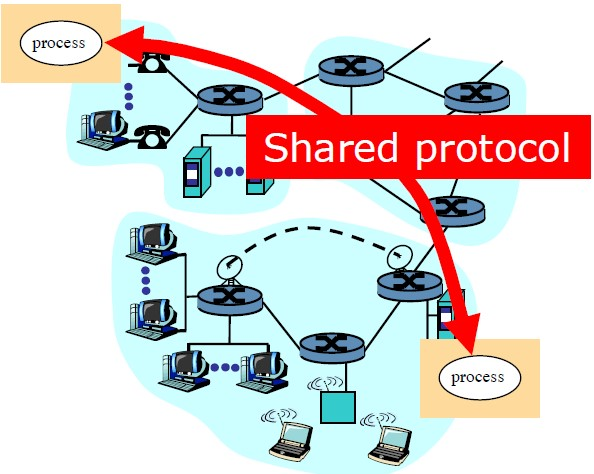
\includegraphics[width=0.675\textwidth]{img/MOC_protocolli1.jpg}
\end{center}

\subsection{Il Web: protocollo http}
http: hypertext transfer protocol
\\Protocollo di livello applicativo per il Web
\\Usa il modello client/server
\begin{itemize}
    \item client: browser che richiede, riceve e “mostra” oggetti Web
    \item server: Web server che invia oggetti in risposta alle richieste
\end{itemize}
\begin{center}
    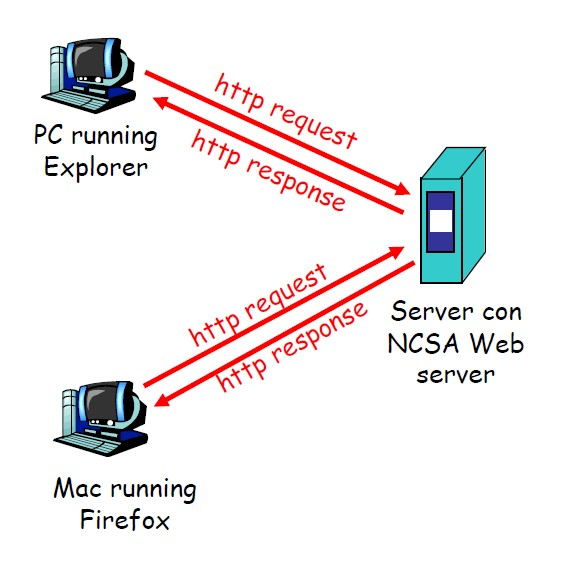
\includegraphics[width=0.5\textwidth]{img/MOC_protocolli2.jpg}
\end{center}
http1.0: RFC 1945
\\http1.1: RFC 2068

\subsubsection{http usa TCP}
Il client inizia una connessione TCP (crea una socket) verso il server sulla porta 80.
\\Il server accetta la connesione TCP dal client
\\Vengono scambiati messaggi http (messaggi del protocollo di livello applicativo) tra il browser (client http) e il Web server (server http).

\subsubsection{http è "stateless"}
Il server non mantiene informazione sulle richieste precedenti del client.
\\Quindi: ogni richiesta deve contenere tutte le informazioni necessarie per la sua esecuzione.
\\I protocolli che mantengono informazione di stato sono complessi (es. TCP)!

\subsection{Formato dei messagi http}
Due tipi di messaggi http: \textbf{\textit{request}}, \textbf{\textit{response}}.
\begin{itemize}
    \item ASCII (formato testo leggibile)
    \item Hanno la stessa struttura!
\end{itemize}
\begin{center}
    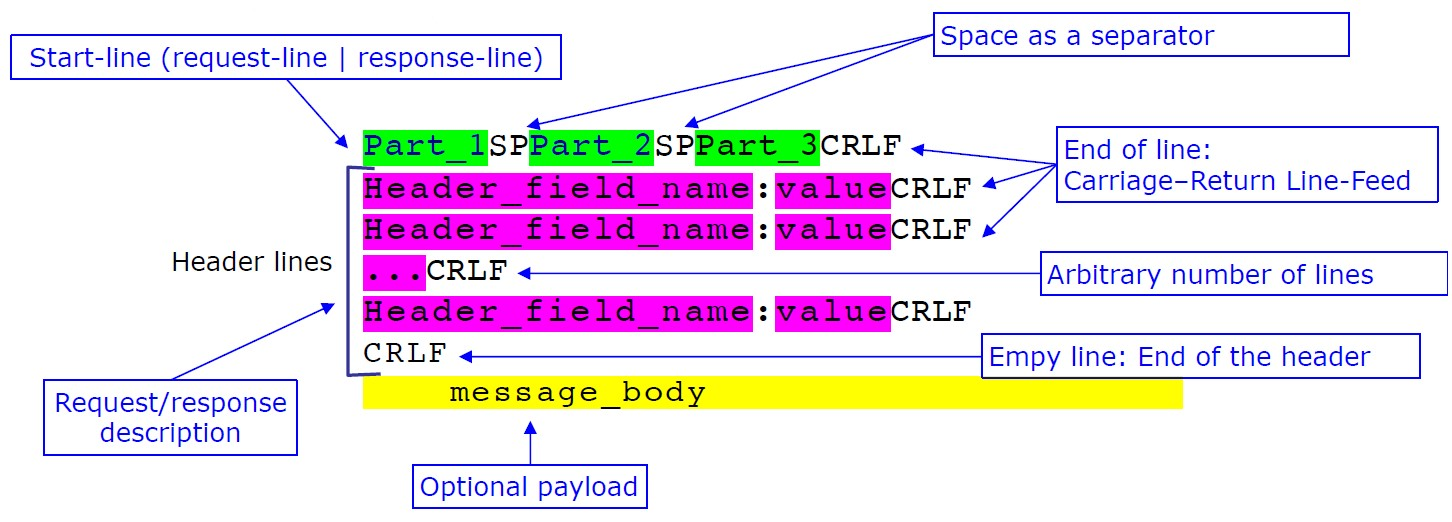
\includegraphics[width=0.5\textwidth]{img/MOC_messaggi1.jpg}
\end{center}
Messaggio http request
\begin{center}
    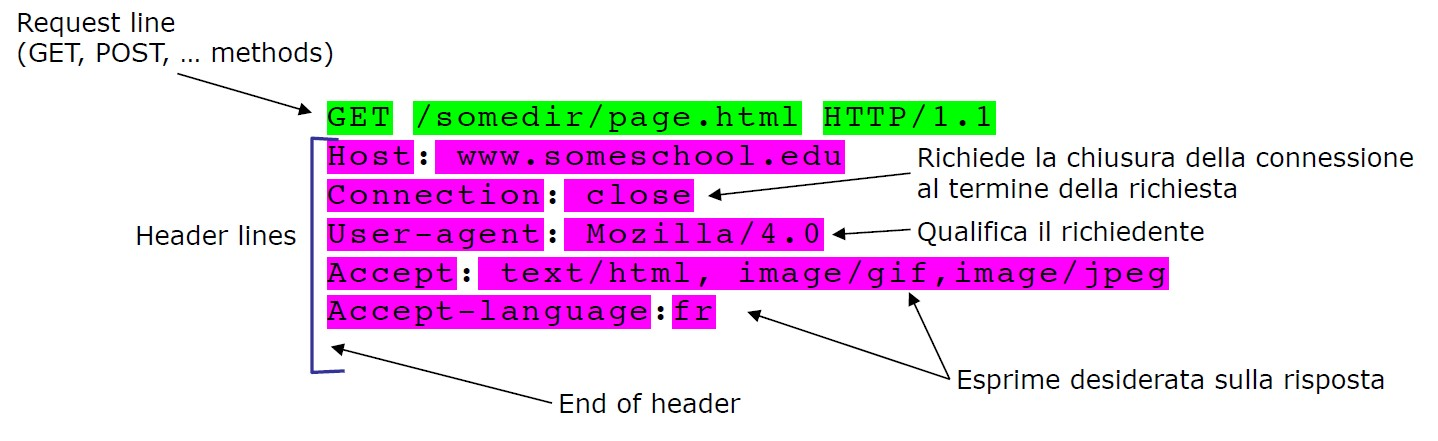
\includegraphics[width=0.5\textwidth]{img/MOC_messaggi2.jpg}
\end{center}

\subsection{Metodi e applicazioni web}
I principali metodi utilizzati sono:
\subsubsection{Metodo GET}
\begin{itemize}
    \item Restituisce una rappresentazione di una risorsa
    \item Include eventuali parametri in coda alla URL della risorsa (vedi più avanti)
    \item \`E safe: l'esecuzione non ha effetti sul server => la risposta può essere gestita con una cache dal client
    \item Uso tipico: ottenere dati in formato di pagine html e immagini, dati XML o JSON
\end{itemize}
La GET include eventuali parametri in coda alla URL della risorsa
\begin{verbatim}
    GET resource[?key=value{&key=value}] HTTP1.1
    {header lines}
\end{verbatim}
Esempio: dammi tutti gli ordini di marzo per il prodotto con codice Q2345
\begin{verbatim}
    /myCompany/orders?item="Q2345"&date="2022/03"
\end{verbatim}
\subsubsection{Metodo POST}
\begin{itemize}
    \item Comunica dei dati da elaborare lato server o crea una nuova risorsa subordinata all'URL indicata (vedi più avanti)
    \item L'input segue come documento autonomo (body)
    \item Non è idempotente: ogni esecuzione ha un diverso effetto => La risposta NON può essere gestita con una cache dal client
    \item Uso tipico: processare FORM e modificare dati in un DB
\end{itemize}
La POST prevede l'input in coda come documento autonomo (body)
\begin{verbatim}
    POST resource HTTP1.1
    {header lines}
    Body
\end{verbatim}
Esempio: aggiorna i codici di un prodotto in tutti gli ordini di aprile
\begin{verbatim}
    POST /myCompany/orders HTTP1.1
    {header lines}
    update=true&oldItem="Q2345"&newItem="Q68254"&date="2022/04"
\end{verbatim}
\subsubsection{Metodo HEAD}
\begin{itemize}
    \item Simile al metodo GET ma viene restituito solo l'Head della pagina Web
    \item Spesso usato in fase di debugging
\end{itemize}

\subsection{Metodi HTTP}
\begin{center}
    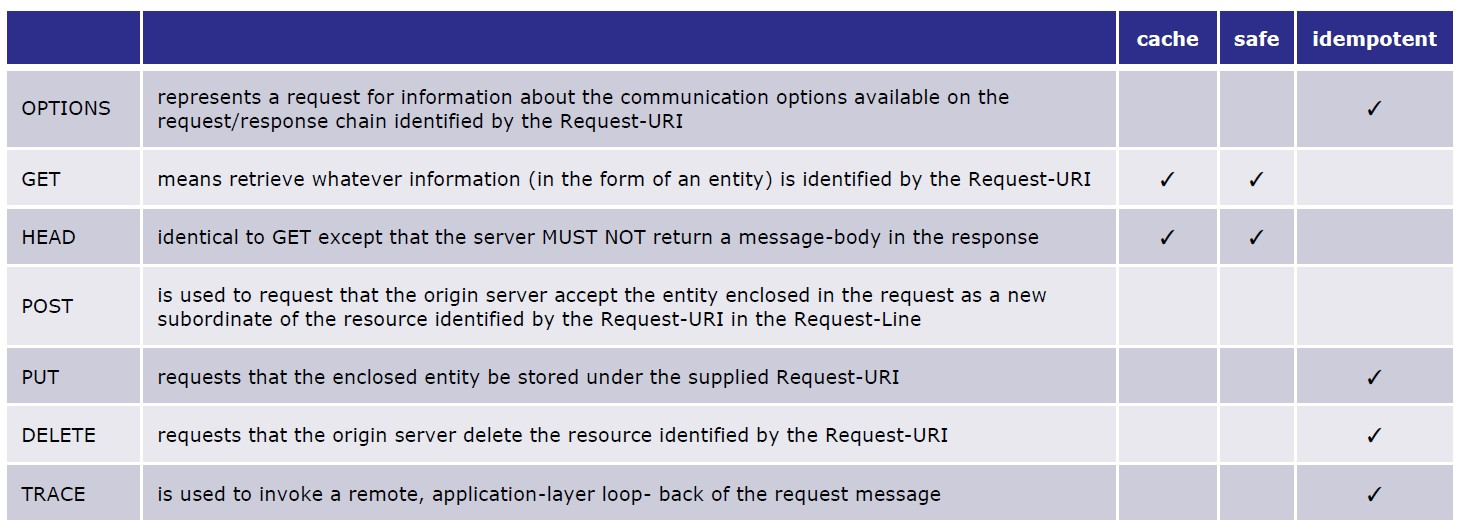
\includegraphics[width=0.675\textwidth]{img/MOC_metodi1.jpg}
\end{center}
\textbf{Safe} = methods SHOULD NOT have the significance of taking an action other than retrieval.
\\\textbf{Idempotent} = the side-effects of N > 0 identical requests is the same as for a single request (aside from error or expiration issues).

\subsection{Formato dei messaggi http}
Messaggio http response
\begin{center}
    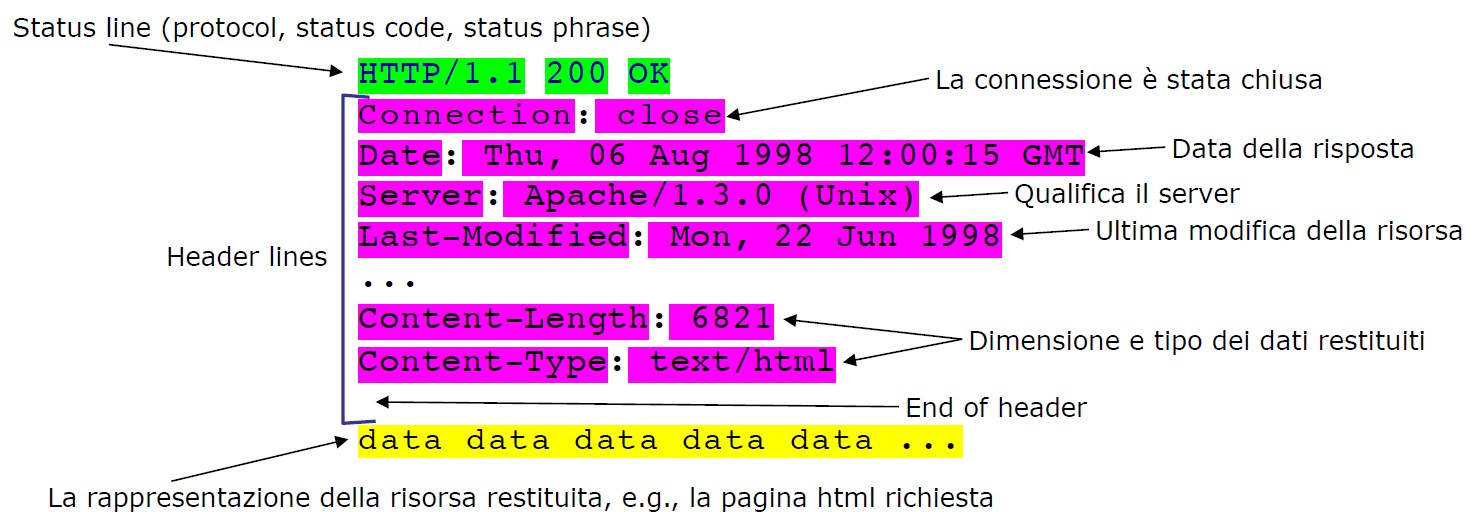
\includegraphics[width=0.675\textwidth]{img/MOC_messaggi3.jpg}
\end{center}
HTTP 1.0: Server chiude connessione al termine della richiesta
\\HTTP 1.1: mantiene aperta la connessione oppure chiude se la richiesta contiene Connection: close
\\
\\Domanda:
\\Perché sono state inserite le informazioni sulla dimensione e il tipo dei dati restituiti?
\begin{verbatim}
    Content-Length: 6812
    Content-Type: text/html
\end{verbatim}









\chapter{Modelli - intro}
\section{Modello dei dati}
Un modello dei dati è un insieme di concetti per organizzare i dati e descriverne la struttura.
\\Questo modello deve essere comprensibile a un elaboratore.
\\Componente fondamentale di ogni modello sono i meccanismi di strutturazione (analogo dei costruttori di tipo).
\\Ogni modello dei dati prevede alcuni costruttori che permettono di definire nuovi tipi sulla base di tipi predefiniti (elementari).
\\Il modello relazionale è il modello di dati più diffuso.

\subsection{Architettura (semplificata) di un DBMS}
\begin{description}
    \item[Schema logico:] descrizione della base di dati nel modello logico adottato (ad esempio, la struttura della tabella).
    \item[Schema interno (o fisico):] rappresentazione dello schema logico per mezzo di strutture di memorizzazione (realizzazione fisica attraverso file; ad esempio, record con puntatori, ordinati in un certo modo)
\end{description}
\begin{center}
    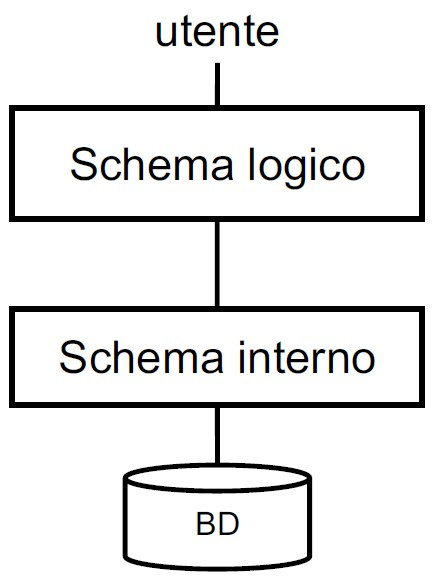
\includegraphics[width=0.5\textwidth]{chaptersLezioniSara/img/MR_intro2.jpg}
\end{center}

\subsection{Indipendenza dei dati}
Il livello logico è \textbf{indipendente} da quello fisico:
\begin{itemize}
    \item una tabella è utilizzata nello stesso modo qualunque sia la sua realizzazione fisica (che può anche cambiare nel tempo)
    \item Perciò in questo corso vedremo solo il livello logico e non quello fisico
\end{itemize}

\subsection{I modelli logici dei dati}
Tre modelli logici tradizionali:
\begin{description}
    \item[gerarchico:] organizzazione ad albero
    \item[reticolare:] organizzazione a grafo
    \item[relazionale:] organizzazione a tabella
\end{description}
Più recenti (e meno diffusi):
\begin{description}
    \item[oggettuale:] organizzazione ad oggetti
    \item[XML] 
    \item[NoSQL:] basata su documenti
\end{description}
Si chiamano modelli \underline{logici} perché pur basandosi su strutture astratte queste riflettono una particolare organizzazione.
\\https://db-engines.com/en/ranking


\subsection{Il modello relazionale}
Permette di definire tipi per mezzo del costruttore \textbf{relazione} che permette di organizzare i dati in insiemi di record a \textit{struttura fissa}.
\\Una relazione è spesso rappresentata da una \textbf{tabella} (solo in questo specifico caso usabile come sinonimo di \textbf{relazione}):
\begin{itemize}
    \item le righe: rappresentano specifici record
    \item le colonne: corrispondono ai campi dei record
\end{itemize}
L'ordine di righe e colonne è sostanzialmente \textit{irrilevante}.
\begin{center}
    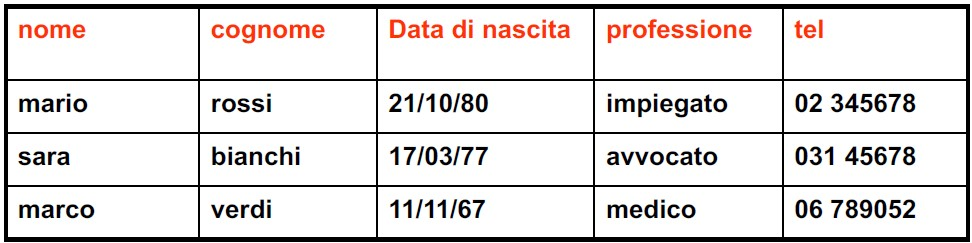
\includegraphics[width=0.5\textwidth]{chaptersLezioniSara/img/MR_intro1.jpg}
\end{center}
In una base di dati relazionale ci sono in generale più relazioni.

\subsubsection{Un po' di storia}
Proposto da E. F. Codd nel 1970 per favorire \textit{l'indipendenza dei dati}.
\\Disponibile in DBMS reali nel 1981 (non è facile implementare l'indipendenza con efficienza e affidabilità!)
\\Basato:
\begin{itemize}
    \item sul concetto matematico di relazione - concetto formale (con una variante)
    \item tabelle - concetto intuitivo
\end{itemize}
Definisce come sono organizzati i dati e non come sono poi memorizzati e gestiti dal sistema informatico.

\subsection{Termine "relazione" in tre accezioni}
\begin{description}
    \item[relazione matematica:] come nella teoria degli insiemi
    \item[relazione:] secondo il modello relazionale dei dati
    \item[associazione o correlazione:] relazione (dall'inglese \textit{relationship}) che rappresenta una classe di fatti, nel modello Entity-Relationship.   
\end{description}

\chapter{Modello Relazionale - MR}
\section{}
\subsection{Prodotto Cartesiano}
Dati due insiemi $D_1, D_2$ (Estendibile a $n$ insiemi distinti o non), definiamo nei seguenti modi:
\begin{itemize}
    \item Prodotto cartesiano $D_1 \times D_2$:
    \\L'insieme di tutte le coppie \textbf{ordinate} $(v_1, v_2)$ tali che $v_1 \in D_1$ e $v_2 \in D_2$
    \item Esempio $$A = {1,\, 2,\, 4}\, e\, B = {a,\, b}$$ Il prodotto cartesiano $A \times B$ è composto da: $${(1,a), (1,b), (2,a), (2,b), (3,a), (3,b)},$$ ovvero sei coppie ordinate (il primo da A, il secondo da B) senza ripetizioni.
\end{itemize}

\subsection{Relazione matematica}
\begin{itemize}
    \item $D1, \dots, Dn$ ($n$ insiemi anche non distinti)
    \item prodotto cartesiano $D_1 \times \cdot \times D_n$:
    \\l'insieme di tutte le $n$-uple ordinate $(d_1, \cdot, d_n)$ tali che $d_1 \in D_1, \cdot, d_n \in D_n$
    \item relazione matematica su $D_1, \cdot, D_n$:
    \\un sottoinsieme di $D_1 \times \cdot \times D_n$, ovvero del prodotto cartesiano.
    \item $D_1, \cdot, D_n$ sono i domini della relazione
\end{itemize}
Il numero delle componenti del prodotto ($n$) è detto \textbf{grado} della relazione; il numero di $n$-uple della relazione è la \textbf{cardinalità} della relazione.

\subsubsection{Es.:}

\subsubsection{Es. numeri di telefono:}

\subsubsection{Rel. matematica: alcune proprietà}
Una relazione matematica è un insieme di n-uple ordinate: (d1, …, dn) tali che d1ÎD1, …, dn Î Dn
\\Alcune proprietà:
\begin{itemize}
    \item non c'è ordinamento fra le n-uple (in verticale);
    \item le n-uple sono distinte;
    \item ciascuna n-upla è ordinata (in orizzontale): l'i-esimo valore proviene dall'i-esimo dominio.
\end{itemize}
L'ultima proprietà ci dice che ciascuno dei domini ha due ruoli diversi, distinguibili attraverso la posizione: ovvero, la struttura è \textbf{posizionale}. Scambiare la posizione fa variare il risultato, portando quindi a possibili errori.
\\Questo si può sistemare aggiungendo alla tabella una riga di \textbf{intestazione}:
\begin{itemize}
    \item a ciascun dominio si associa un nome (attributo), che ne descrive il "ruolo";
    \item gli attributi possono essere usati come intestazione;
    \item la struttura in questo modo non è più posizionale.
\end{itemize}

\subsection{Modello basato su valori}
Immagine
\subsubsection{Vantaggi:}
Indipendenza dalle strutture fisiche (si potrebbe avere anche 
con puntatori di alto livello) che possono cambiare
dinamicamente
• si rappresenta solo ciò che è rilevante dal punto di vista
dell'applicazione
• i dati sono portabili piu' facilmente da un sistema ad un altro
• per accedere ai dati non serve sapere come sono memorizzati
fisicamente
\subsection{Modello basato su puntatori}
Immagine

\subsection{Schema e istanza}
In ogni base di dati esistono:
• lo schema, sostanzialmente invariante nel tempo, che ne
descrive la struttura (aspetto intensionale). Scritto con la lettera maiuscola.
• es.: le intestazioni delle tabelle
• l'istanza, i valori attuali, che possono cambiare anche
molto rapidamente (aspetto estensionale). Scritto con la lettera minuscola.
• es.: il “corpo” di ciascuna tabella

\subsubsection{Definizioni}
Schema di relazione:
un nome R1 (MAIUSCOLO) con un insieme di attributi
X={A1, ..., An}:
R1(A1,..., An) = R1(X)
% immagine
Schema di base di dati:
insieme di schemi di relazione con nomi diversi:
R = {R1(X1), ..., Rk(Xk)}
% immagine
Una tupla su un insieme di attributi X è una funzione t che associa a
ciascun attributo A in X un valore del dominio di A
• t[A] (o t.A) denota il valore della tupla t sull'attributo A
% immagine
una relazione R con attributi A1, A2 e A3, e corrispondenti
domini D1, D2 e D3 si può denotare anche come
R(A1 : D1, A2 : D2, A3 : D3)

(Istanza di) relazione su uno schema R(X):
insieme r1 (minuscolo) di tuple su X
• (Istanza di) base di dati su uno schema R= {R1(X1), ..., Rn(Xn)}:
insieme di relazioni r = {r1,..., rn} (con ri relazione su Ri)

\subsection{Un po' di notazione}


\subsection{Tabelle e relazioni}
Una tabella rappresenta una relazione se
\begin{itemize}
    \item i valori di ogni colonna sono fra loro omogenei
    \item le righe sono diverse fra loro
    \item le intestazioni delle colonne sono diverse tra loro
\end{itemize}
In una tabella che rappresenta una relazione
\begin{itemize}
    \item l'ordinamento tra le righe è irrilevante
    \item l'ordinamento tra le colonne è irrilevante
\end{itemize}

\subsubsection{Chiave}
insieme di attributi che identificano univocamente le tuple di
una relazione
Formalmente:
• un insieme K di attributi è superchiave per r se r non
contiene due tuple distinte t1 e t2 con t1[K] = t2[K]
• K é chiave per r se è una superchiave minimale per r (cioé non contiene un'altra superchiave)
% tre esempi
Ma data una tabella qualsiasi, esiste sempre una superchiave (\textbf{NON} minimale)? Dato che la tabella proviene da un prodotto cartesiano e nel prodotto cartesiano non ci sono ripetizioni, allora possiamo dire che la risposta è sì. E la superchiave corrisponderà all'insieme di \textbf{tutti} gli attributi della tanella.
\\All'esame ci verranno dati schemi di relazione, dobbiamo individuarne la superchiave e i vincoli.

\subsubsection{Informazione incompleta}
ll modello relazionale impone ai dati una struttura rigida:
\begin{itemize}
    \item le informazioni sono rappresentate per mezzo di tuple
    \item solo alcuni formati di tuple sono ammessi: quelli che corrispondono agli schemi di relazione
\end{itemize}
I dati disponibili possono non corrispondere al formato previsto:
\begin{itemize}
    \item Hanno attributi in più che non sono nello schema
    \item Mancano di alcuni attributi = Informazione incompleta
\end{itemize}

\subsubsection{Informazione incompleta: motivazioni}
% immagine

\subsubsection{Informazione incompleta nel modello relazionale}
Si adotta una tecnica rudimentale ma efficace:
• valore nullo: denota l'assenza di un valore del dominio
(e non è un valore del dominio)
• t[A], per ogni attributo A, è un valore del dominio dom(A)
oppure il valore nullo NULL

e altre cose

tutti questi vincoli ci aiutano a gestire la bd in modo che i dati non siano incosistenti.

tipi di vincoli:

per la slide 61, all'esame va bene così com'è nella slide oppure in linguaggio naturale

\section{Ricapitolazione di quanto visto finora}
\begin{description}
    \item[Modello relazionale]
    \item[Concetto relazione come variazione] (attributi, campi) di relazione matematica (tabella)
    \item[Schema e istanza:] $R(A_1, A_2, ..., A_n)$ per la relazione, $r(a_1, a_2, ..., a_n)$ per le istanze
    \item[Basi di dati come insieme di relazioni] $R = {(A_1, A_2, ..., A_n)}$
    \item[Superchiave:] insieme di attributi per cui la relazione R di cui è superchiave in cui non c'è nessuna tupla che si ripete. L'insieme di tutti gli attributi di una relazione è un esempio di superchiave.
    \item[Superchiave minimale (o CHIAVE):] quella che non contiene nessun'altra sottochiave, o nessun altro sottoinsieme di attributi.
    \item[Valore nullo:] "null", esiste per alcuni attributi, mentre altri non possono avere valore nullo; è un po' come facevamo in E-R, quando mettavamo cardinalità (0, 1) per un attributo in modo da indicarne l'opzionalità.
    \item[Vincoli di inter e intra relazionali:] vedremo oggi
    \item[Chiave Primaria:] vedremo oggi
\end{description}

\section{Tipi di vincoli}
\begin{description}
    \item[vincoli intrarelazionali:]
    \item vincoli su valori (o di dominio)
    \item vincoli di tupla
    \item vincoli di chiave (valuta le tuple nel complesso. es. non possono esistere due tuple con uno stesso valore per un particolare attributo A chiave).
    \item[vincoli interrelazionali] (coinvolge più relazioni): 
    \item vincoli di integrità referenziale
\end{description}
Tre concetti:
\begin{itemize}
    \item superchiave
    \item superchiave minimale (o Chiave)
    \item Chiave primaria
\end{itemize}
La \textbf{chiave primaria} non contiene attributi nulli. Sottoinsieme di attributi per cui è impossibile definire una superchiave minimale e per cui è impossibile avere attributi nulli.
\\Es.: tabella pag 65 universitari: la tabella avrà sempre una superchiave minimale, la matricola, che non può avere valore nullo (altrimenti come li identifichiamo gli studenti?) e questa è la \textbf{chiave primaria}.

\subsection{Importanza delle chiavi}
L'esistenza delle chiavi garantisce l'accessibilità a ciascun dato della base di dati.
\\Le chiavi permettono di correlare i dati in relazioni diverse: il modello relazionale è basato su valori.
\begin{center}
    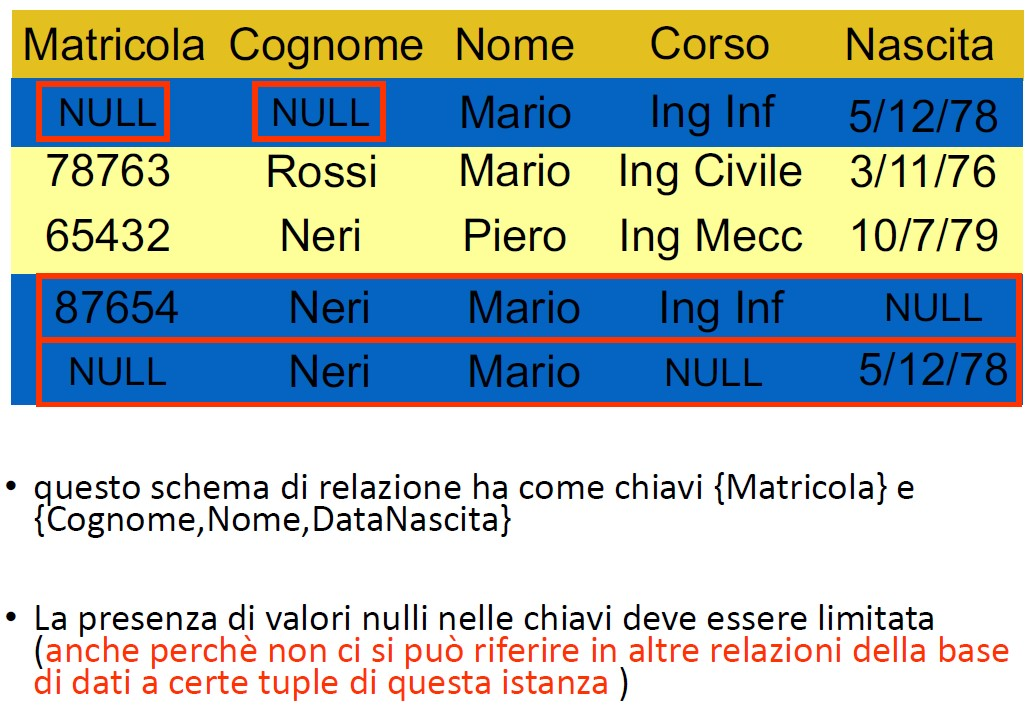
\includegraphics[width=0.5\textwidth]{chaptersLezioniSara/img/MR_chiavi777.jpg}
\end{center}
La slide 71 mi riporta un esempio in cui i dati sono rappresentati in 3 tabelle scorrelate e relativamente indipendenti fra loro. Nella slide successiva viene mostrato l'output che avremmo se provassimo a rappresentare i dati in una sola tabella. Che non funzionerebbe tanto perché ci sarebbero troppe ripetizioni e poi avremmo anche molti valori nulli. Questa rappresentazione era da citare però perché mostra il comportamento di NoSQL.

\section{Vincolo di integrità referenziale}
Un \textbf{vincolo di integrità referenziale} (\textit{"foreign key"}) fra gli attributi $X$ di una relazione $R_1$ e un'altra relazione $R_2$ impone ai valori su $X$ in $R_1$ di comparire come valori della chiave primaria di $R_2$.
\\All'esame dovremo scegliere noi la chiave primaria (sottolineandola) e dire quali attributi vanno a formare il vincolo, ovvero a comporre la chiave primaria.
\begin{center}
    \includegraphics[width=0.5\textwidth]{chaptersLezioniSara/img/MR_integrità_referenziale1.jpg}
\end{center}
\begin{center}
    \includegraphics[width=0.5\textwidth]{chaptersLezioniSara/img/MR_integrità_referenziale2.jpg}
\end{center}
Leggi tu le slide, ora un esercizio di esempio.

\section{Esercizi di esempio}
\subsection{Es.: prestito di libri}
\begin{center}
    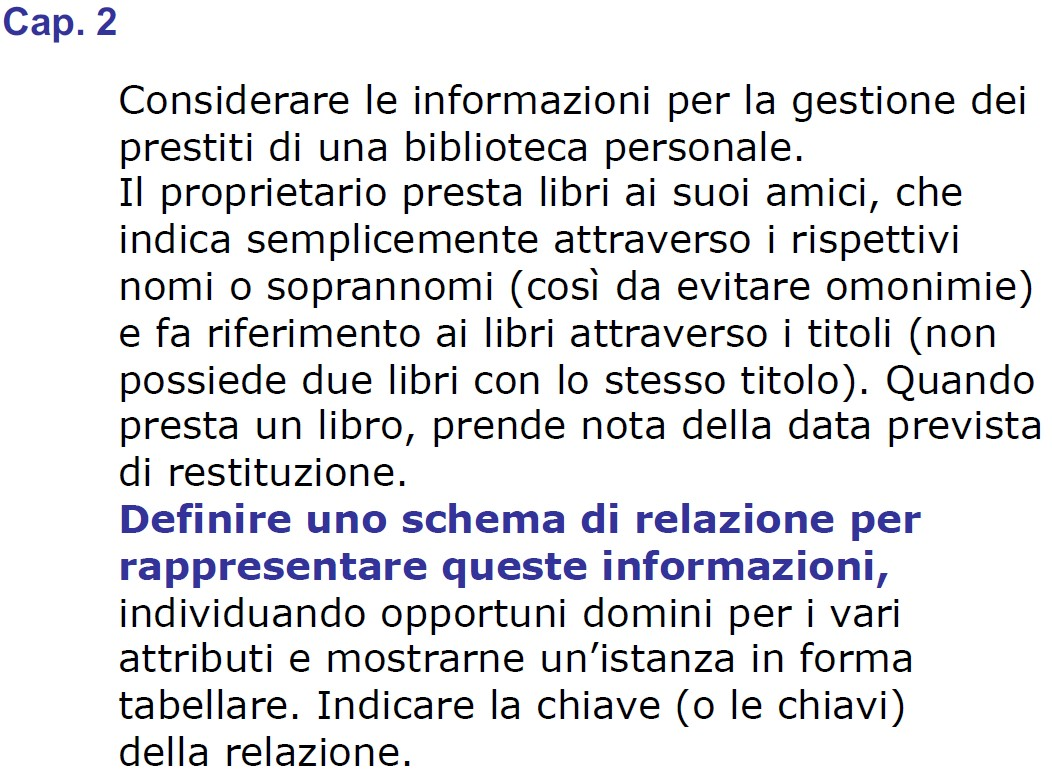
\includegraphics[width=0.5\textwidth]{chaptersLezioniSara/img/MR_es_prestitolibri1.jpg}
\end{center}
Quello che dobbiamo fare noi è scegliere la chiave primaria e dire quali attributi vanno a formare il vincolo, ovvero a comporre la chiave primaria.
\begin{center}
    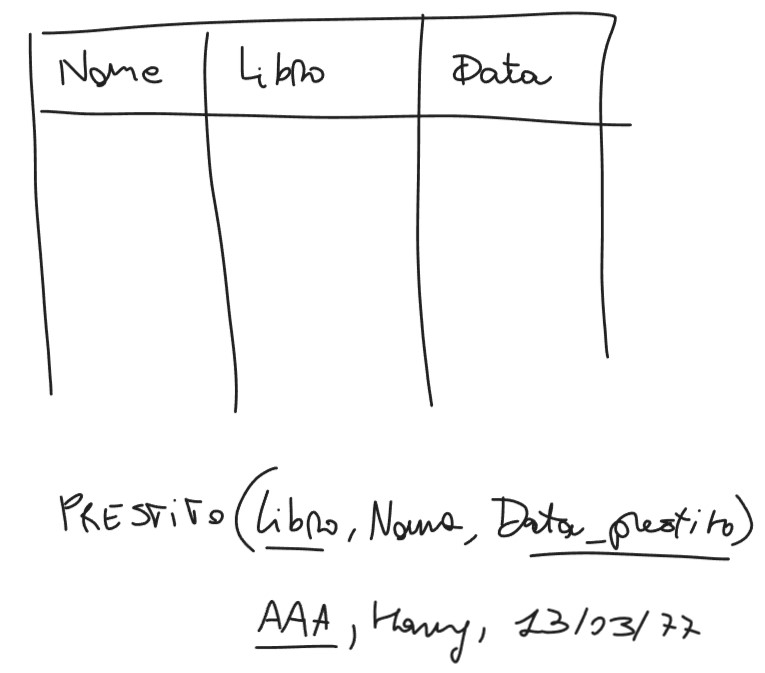
\includegraphics[width=0.5\textwidth]{chaptersLezioniSara/img/MR_es_prestitolibri2.jpg}
\end{center}
\begin{center}
    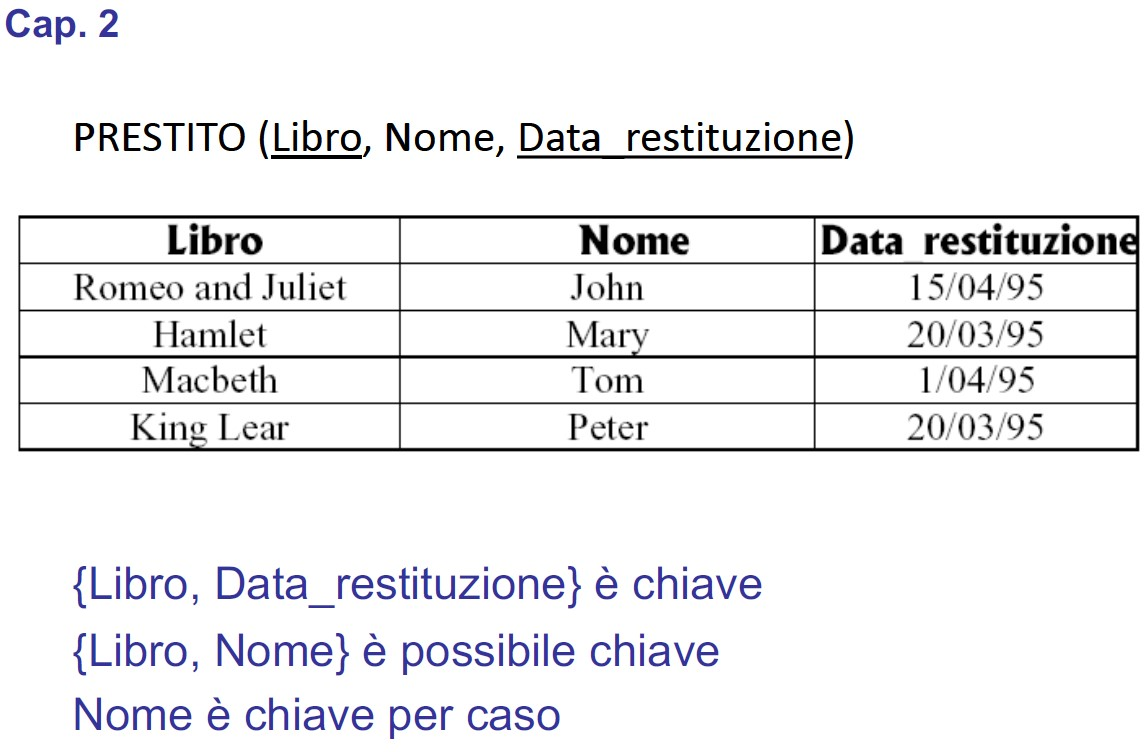
\includegraphics[width=0.5\textwidth]{chaptersLezioniSara/img/MR_es_prestitolibri3.jpg} 
\end{center}

\subsection{Altro esempio}
Facciamo una sorta di reverse ingeniering: prendiamo una tabella e cerchiamo di capire come è stata fatta.
\\Ovvero: descrivere in linguaggio naturale le informazioni organizzate nella base di dati. 
Individuare: 
\begin{enumerate}
    \item le chiavi (primaria, e almeno 1 superchiave)
    \item i vincoli di integrità referenziale
    \item gli attributi su cui NON possono essere ammessi valori nulli.
\end{enumerate} 
Per il punto 1.:
\begin{center}
    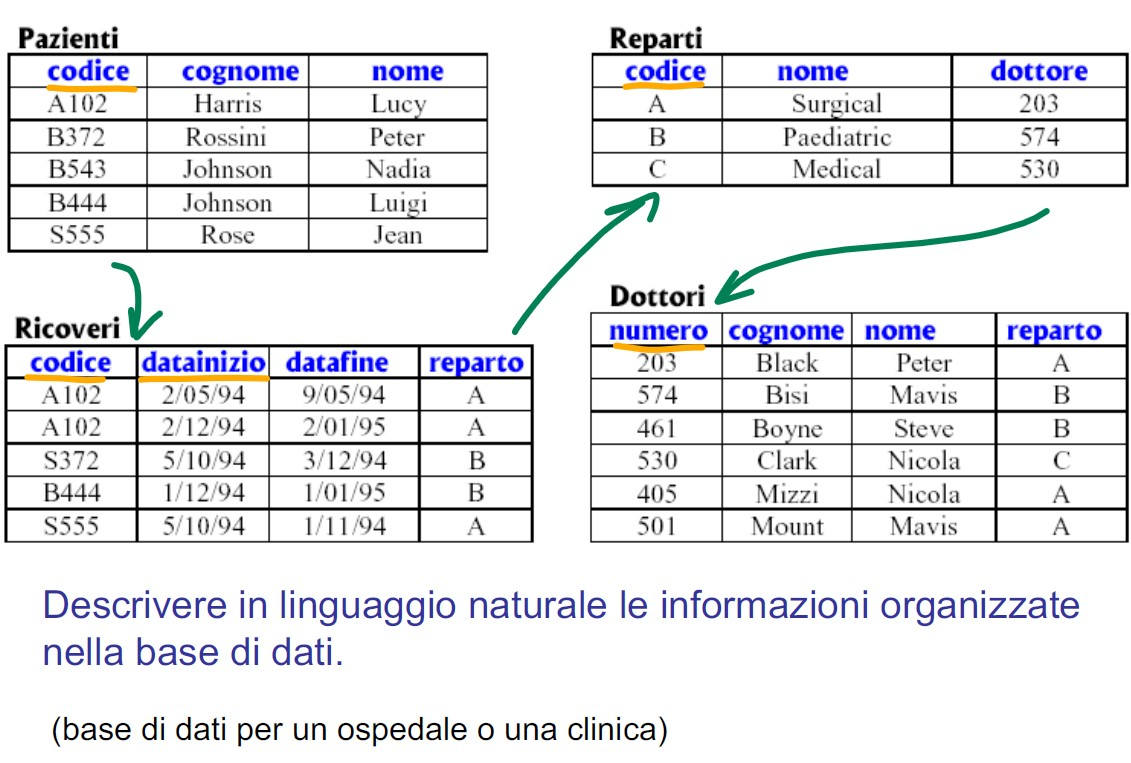
\includegraphics[width=0.5\textwidth]{chaptersLezioniSara/img/MR_es_altro1.jpg}
\end{center}
Per il punto 2.: c'è un vincolo di integrità referenziale non rispettato (ovvero, non esiste nella tabella dei pazienti il paziente identificato dal codice S372 che è possibile vedere nella tabella dei ricoveri).
\\Per il punto 3.: tutte le chiavi primarie ovviamente.

\subsubsection{Soluzioni}
\begin{enumerate}
    \item I valori nulli sono permessi solo negli attributi che non sono chiave primaria.
    \item Alcuni non hanno molto senso (nome cognome in Dottori) 
    \item Codice per la relazione PAZIENTI
    \item {Paziente, datainizio}, {Paziente, datafine} per la relazione RICOVERI (si assume che un paziente sia ricoverato -dimesso- una sola volta in un giorno)
    \item Numero per la relazione DOTTORI
    \item Codice per la relazione REPARTI
    \item I vincoli referenziali sono fra:
    \\• Codice in RICOVERI e Codice in PAZIENTI
    \\•Reparto in RICOVERI e Codice in REPARTI
    \\• Dottore in REPARTO e Numero in DOTTORI
    \\• Reparto in DOTTORI e Codice in REPARTI
    \item I valori nulli sono permessi solo negli attributi che non sono chiave primaria. Alcuni non hanno molto senso (nome cognome in Dottori)
\end{enumerate}

\subsection{Altro esempio: stazione}
\begin{center}
    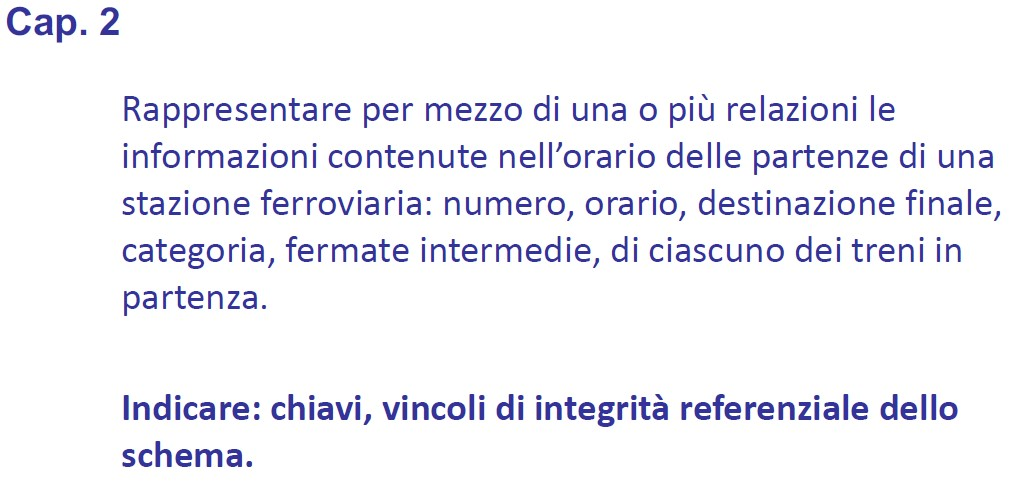
\includegraphics[width=0.5\textwidth]{chaptersLezioniSara/img/MR_es_stazione1.jpg}
\end{center}
Sol. aula:
\begin{verbatim}
    TRENO (Tipo, \underline{Numero}, DestinazioneFinale, OrarioPartenza)
    FERMATE (\underline{Nome, Numero,} Orario)
\end{verbatim}
Sol. slides:
\begin{verbatim}
    PARTENZE (\underline{Numero}, OrarioPartenza, Destinazione Finale, Categoria)
    FERMATE (\underline{Treno, Stazione}, Orario)
\end{verbatim}
La prima relazione rappresenta tutti i treni in partenza dalla stazione ferroviaria, distinti per il Numero (chiave primaria della relazione).
\\La seconda rappresenta le fermate intermedie per ciascun treno in ciascuna stazione (chiave primaria composta da Treno e Stazione) con vincolo referenziale fra Treno in STOP e Numero in PARTENZE.
\\Manca qualcosa: relazione treno.
\begin{verbatim}
    TRENO(\underline{Numero}, Categoria)
\end{verbatim}
La terza rappresenta le fermate intermedie per ciascun treno in ciascuna stazione (chiave primaria composta da Treno, Stazione e orario).

\subsection{Altro esempio: azienda}
\begin{center}
    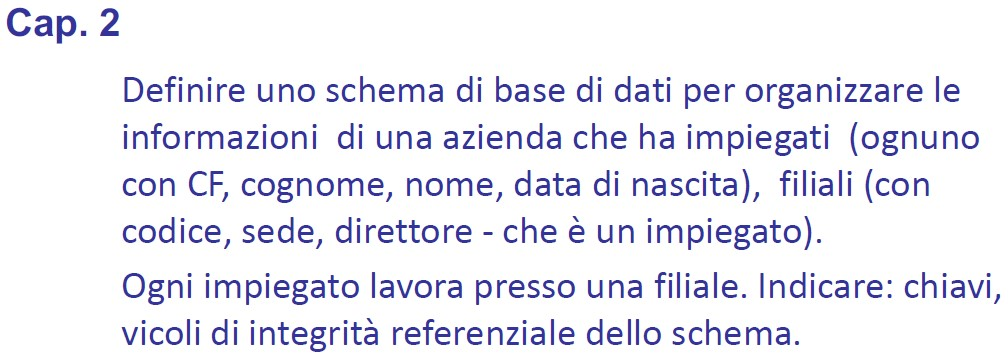
\includegraphics[width=0.5\textwidth]{chaptersLezioniSara/img/MR_es_azienda1.jpg}
\end{center}
Quante relazioni ci servono? 2. Ogni filiale ha più impiegati. Quindi una tabella per filiali, una per impiegati, una per azienda.
\begin{verbatim}
    IMPIEGATO (\underline{CF}, Nome, Cognome, Nascita, Filiale)
    FILIALE (\underline{Codice}, Sede, Direttore)
\end{verbatim}
Ellisse con freccia da IMPIEGATO(..., Filiale) a FILIALE(Codice, ...) per indicare il vincolo di integrità referenziale.
\\Ellisse con freccia da FILIALE(..., Direttore) a IMPIEGATO per indicare il vincolo di integrità referenziale.

\subsection{Altro esempio: radio}
\begin{center}
    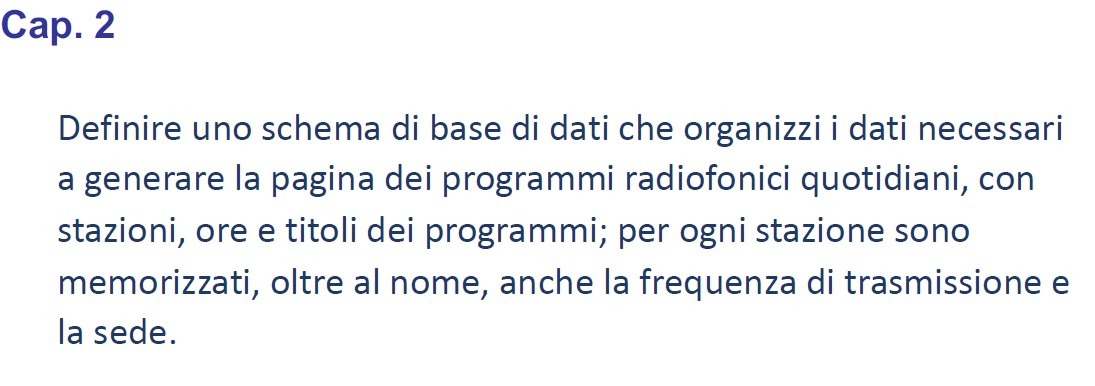
\includegraphics[width=0.5\textwidth]{chaptersLezioniSara/img/MR_es_radio1.jpg}
\end{center}
Quante relazioni ci servono? 2.
\begin{verbatim}
    PROGRAMMI (\underline{Titolo, Stazione}, Orario) 
    STAZIONE (\underline{Nome}, Frequenza, Sede)
\end{verbatim}
Magari all'interno di PROGRAMMI(...) basta da solo il Titolo per identificare univocamente un programma all'interno di una stazione.
\begin{center}
    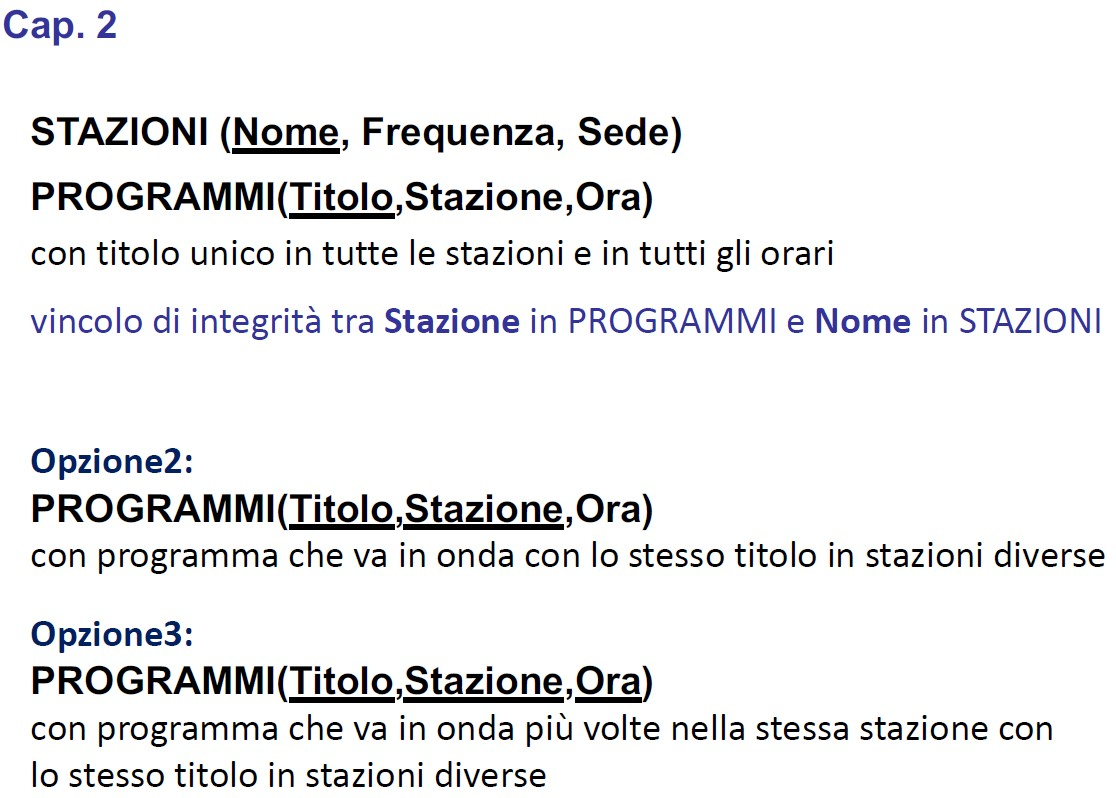
\includegraphics[width=0.5\textwidth]{chaptersLezioniSara/img/MR_es_radio2.jpg}
\end{center}

\section{Esempio di esercizio MR che troveremo all'esame}
\begin{center}
    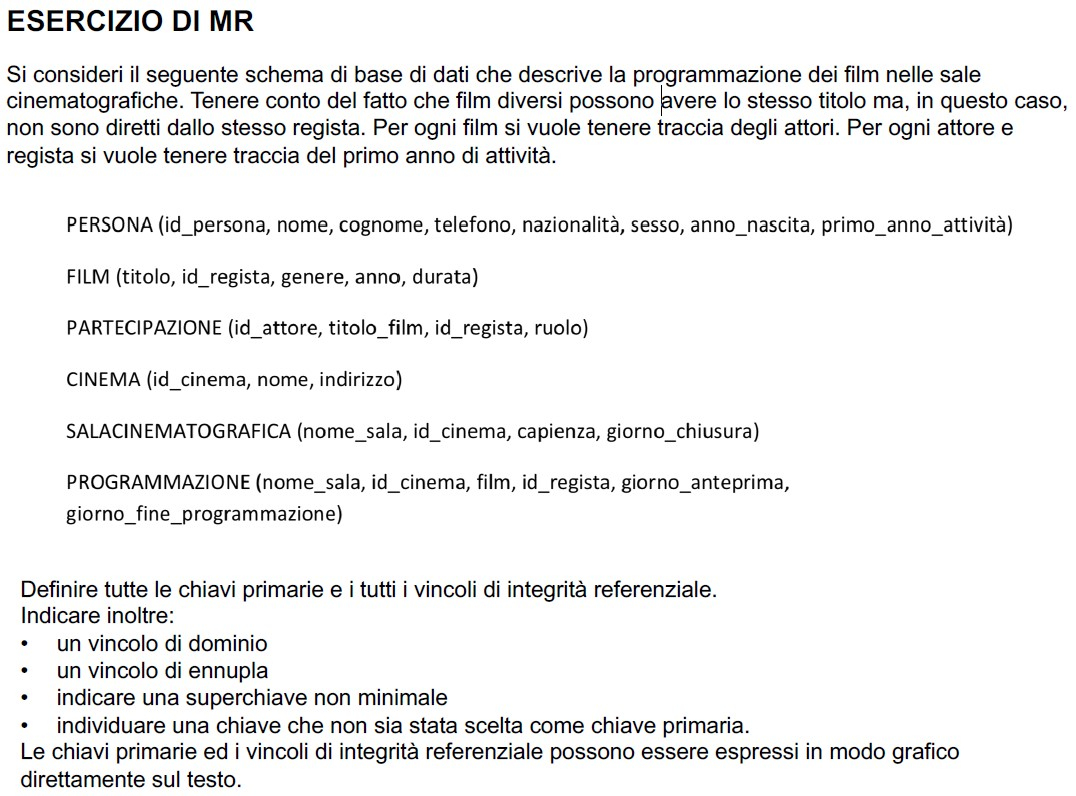
\includegraphics[width=0.5\textwidth]{chaptersLezioniSara/img/MR_facsimile_esame1.jpg}
\end{center}
\begin{center}
    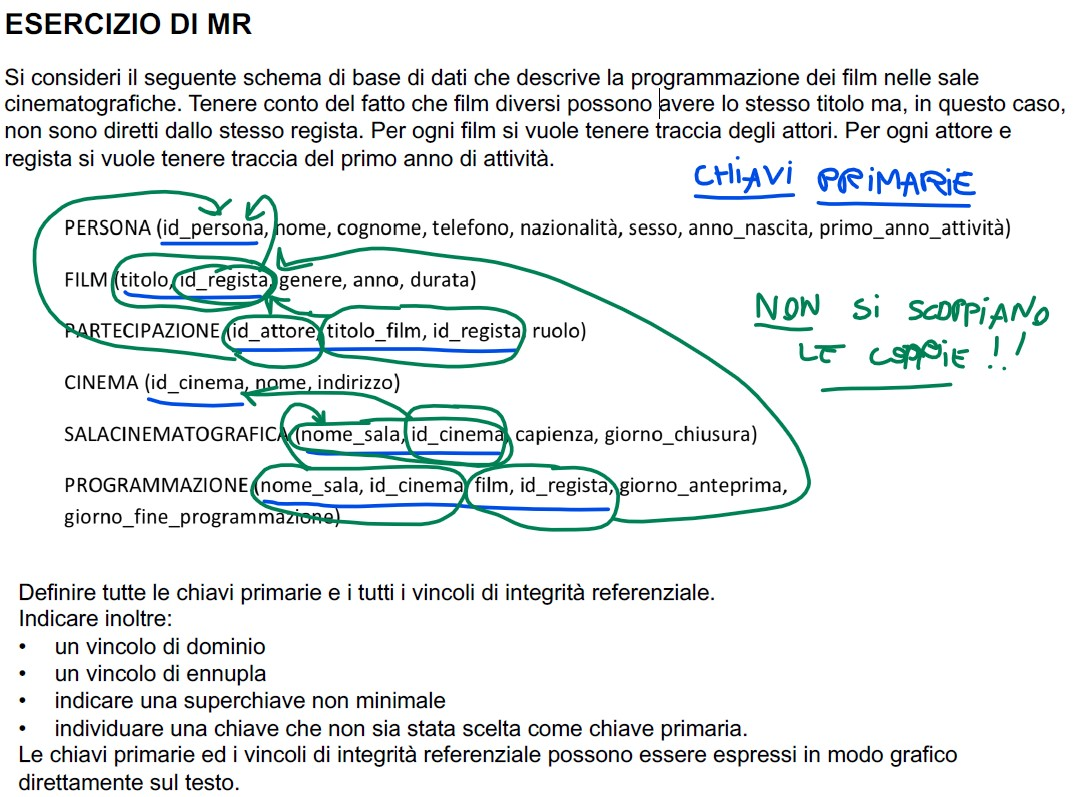
\includegraphics[width=0.5\textwidth]{chaptersLezioniSara/img/MR_facsimile_esame2.jpg}
\end{center}
\begin{center}
    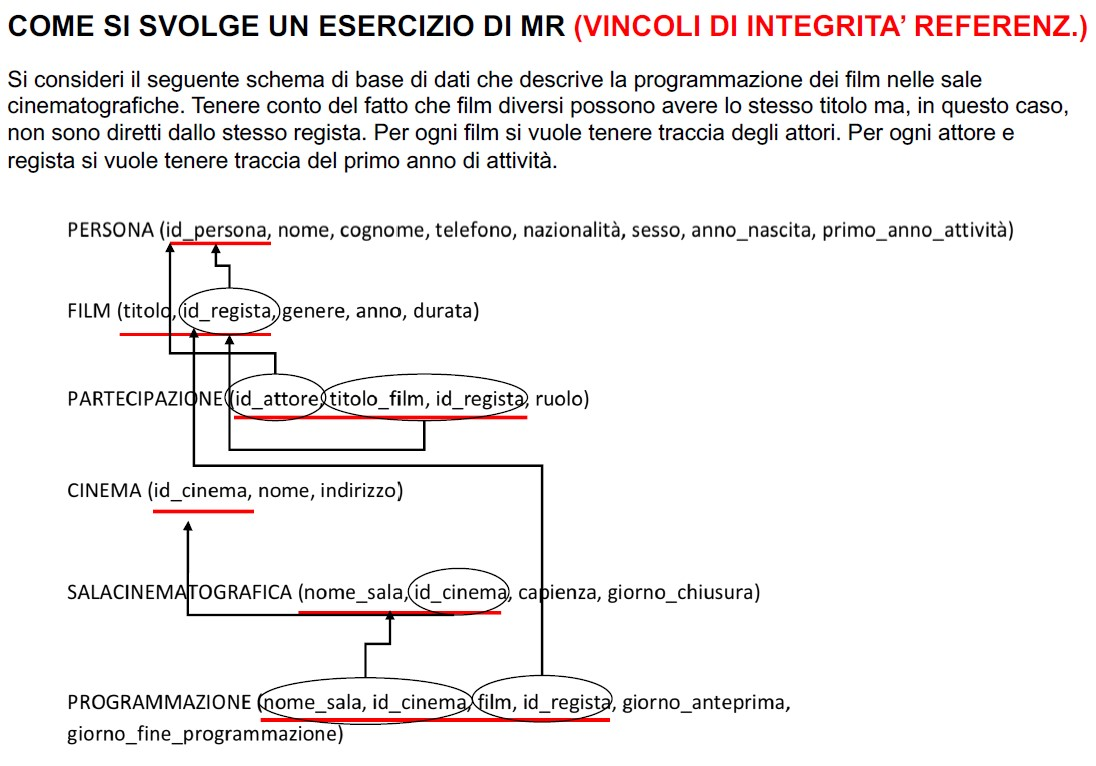
\includegraphics[width=0.5\textwidth]{chaptersLezioniSara/img/MR_facsimile_esame3.jpg}
\end{center}



\chapter{Esercizi di MR}
Svolgere gli esercizi nel seguente modo:
\begin{itemize}
    \item Identificare le relazioni che modellano il dominio descritto nel testo
    \item Identificare per ogni relazione le chiavi primarie e i vincoli di integrità referenziale
    \item Identificare almeno un vincolo di dominio
    \item Identificare quali attributi ammettono valori nulli
    \item Identificare un vincolo di ennupla
    \item Identificare una superchiave
    \item Identificare una chiave alternativa
\end{itemize}

\section{Es. A}
Si consideri il seguente schema di basi di dati che descrive un campionato provinciale di pallavolo. Le squadre si incontrano due volte, nel girone di andata e in quello di ritorno. Si tenga presente che il risultato di una partita di pallavolo è al meglio dei cinque set, non è detto che una squadra giochi le partite nella palestra dove si allena, più squadre possono allenarsi o giocare in giorni/orari diversi ma nella stessa palestra. 

\subsubsection{Identifico le relazioni: attributi}
\begin{itemize}
    \item SQUADRA (nome, capitano, città, palestraAll, cittàAll, palestraPart, cittàPart, sponsor)
    \item PALESTRA (nome, città, indirizzo, numPosti)
    \item ATLETA (tesserino, nome, cognome, dataNascita, luogoNascita, squadra)
    \item ARBITRO (tesserino, nome, cognome, dataNascita, luogoNascita, numPartiteArbitrate)
    \item SPONSOR (pIva, nome, telefono)
    \item RISULTATO (squadraCasa, squadraOspite, setSquadraCasa, setSquadraOspite, arbitro, palestra, città, data, oraInizio, oraFine)
\end{itemize}

\subsubsection{Identifico le chiavi primarie}
\begin{itemize}
    \item SQUADRA (\underline{nome}, capitano, città, \textbf{palestraAll}, cittàAll, palestraPart, cittàPart, sponsor)
    \item PALESTRA (\underline{nome, città}, indirizzo, numPosti)
    \item ATLETA (\underline{tesserino}, nome, cognome, dataNascita, luogoNascita, squadra)
    \item ARBITRO (\underline{tesserino}, nome, cognome, dataNascita, luogoNascita, numPartiteArbitrate)
    \item SPONSOR (\underline{pIva}, nome, telefono)
    \item RISULTATO (\underline{squadraCasa, squadraOspite}, setSquadraCasa, setSquadraOspite, arbitro, palestra, città, data, oraInizio, oraFine)
\end{itemize}

\subsubsection{Identifico gli attributi che possono essere nulli}
\begin{itemize}
    \item SQUADRA (nome, capitano, città, palestraAll, cittàAll, palestraPart, cittàPart, \textit{sponsor})
    \item PALESTRA (nome, città, indirizzo, numPosti)
    \item ATLETA (tesserino, nome, cognome, dataNascita, luogoNascita, squadra)
    \item ARBITRO (tesserino, nome, cognome, dataNascita, luogoNascita, \textit{numPartiteArbitrate})
    \item SPONSOR (pIva, nome, telefono)
    \item RISULTATO (squadraCasa, squadraOspite, \textit{setSquadraCasa, setSquadraOspite}, arbitro, palestra, città, data, oraInizio, oraFine)
\end{itemize}
\begin{center}
    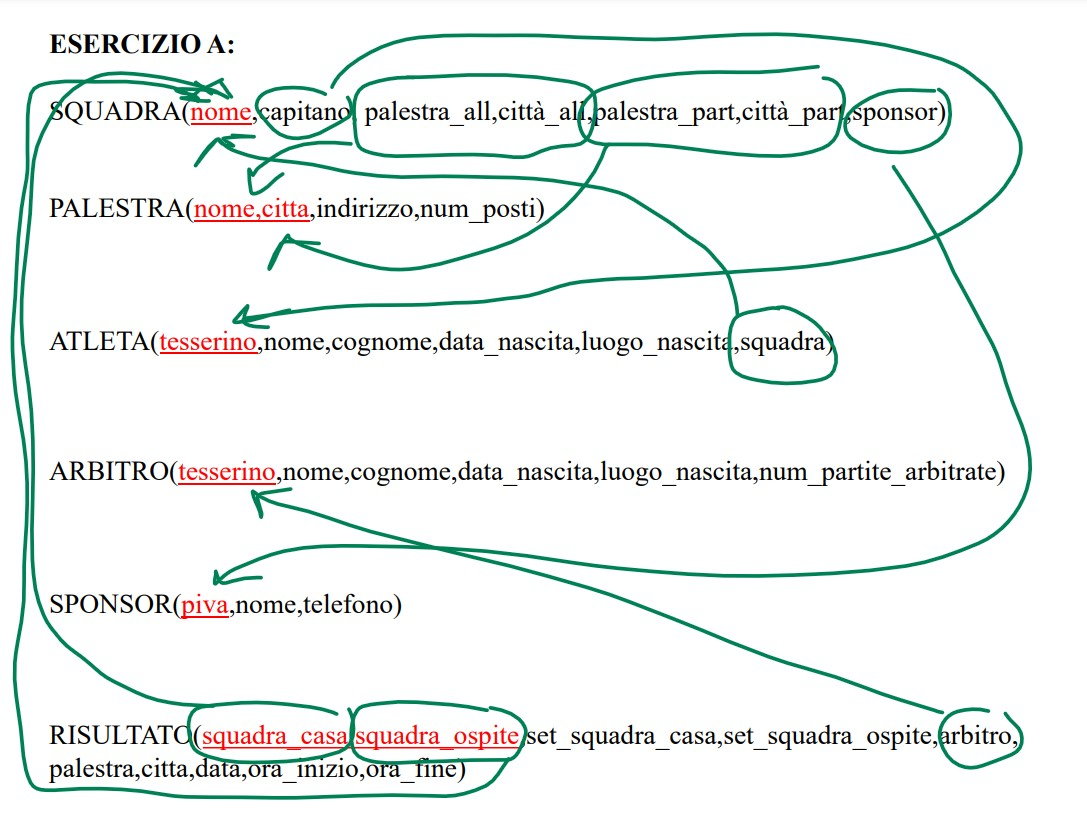
\includegraphics[width=0.675\textwidth]{chaptersLezioniSara/img/MR_fileesA.jpg}
\end{center}

\subsubsection{Identifico i vincoli di tupla}
\begin{itemize}
    \item setSquadraCasa e setSquadraOspite devono essere maggiori uguali di zero e minori uguali di 3.
    \item setSquadraCasa + setSquadraOspite deve essere maggiore uguale di 3 e minore uguale di 5.
    \item oraInizio < oraFine
    \item Una superchiave nella tabella sponsor è p.via, nome, telefono
    \item Una chiave alternativa è numTelefono in sponsor
\end{itemize}

\section{Es. B}
Si consideri il seguente schema di basi di dati che descrive le informazioni relative ad una olimpiade. Per ogni nazione si vuole tenere traccia dell'atleta porta bandiera, del numero di atleti, della mascotte e colore della divisa. Si vuole tenere traccia degli atleti e delle partecipazioni degli atleti alle gare con posizione raggiunta e fase della gara a cui sono arrivati. Per esempio nelle gare di corsa, le fasi possono essere: qualificazioni, ottavi, quarti, ecc. Ogni fase di gara ha due giudici e si svolgono ad una specifica data, ora e luogo. Per ogni atleta si vuole tenere traccia del codice tesserino atleta, nazione, cognome, nome e data di nascita.

\subsubsection{Identifico le relazioni}
\begin{itemize}
    \item NAZIONE (nome, portabandiera, numeroAtleti, mascotte, coloreDivisa)
    \item ATLETA (tesserino, nome, cognome, dataNascita, nazione)
    \item GARA (nomeGara, disciplina, recordMondiale, recordOlimpionico)
    \item SVOLGIMENTOGARA (gara, faseGara, luogo, data, ora, giudice1, giudice2)
    \item PARTECIPAZIONEGARA (atleta, gara, faseGara, posizioneClassifica, datiGara)
    \item GIUDICE (tesserino, nome, cognome, dataNascita, nazione)
\end{itemize}

\subsubsection{Identifico le chiavi primarie}
\begin{itemize}
    \item NAZIONE (\underline{nome}, portabandiera, numeroAtleti, mascotte, coloreDivisa)
    \item ATLETA (\underline{tesserino}, nome, cognome, dataNascita, nazione)
    \item GARA (\underline{nomeGara}, disciplina, recordMondiale, recordOlimpionico)
    \item SVOLGIMENTOGARA (gara, faseGara, luogo, data, ora, giudice1, giudice2)
    \item PARTECIPAZIONEGARA (atleta, gara, faseGara, posizioneClassifica, datiGara)
    \item GIUDICE (tesserino, nome, cognome, dataNascita, nazione)
\end{itemize}

\subsubsection{Identifico gli attributi che possono essere nulli}
Non è che abbia capito molto
\begin{itemize}
    \item NAZIONE (nome, portabandiera, numeroAtleti, mascotte, coloreDivisa)
    \item ATLETA (tesserino, nome, cognome, dataNascita, nazione)
    \item GARA (nomeGara, disciplina, recordMondiale, recordOlimpionico)
    \item SVOLGIMENTOGARA (gara, faseGara, luogo, data, ora, giudice1, \textbf{giudice2})
    \item PARTECIPAZIONEGARA (atleta, gara, faseGara, posizioneClassifica, datiGara)
    \item GIUDICE (tesserino, nome, cognome, dataNascita, nazione)
\end{itemize}
Boh da finire
\begin{center}
    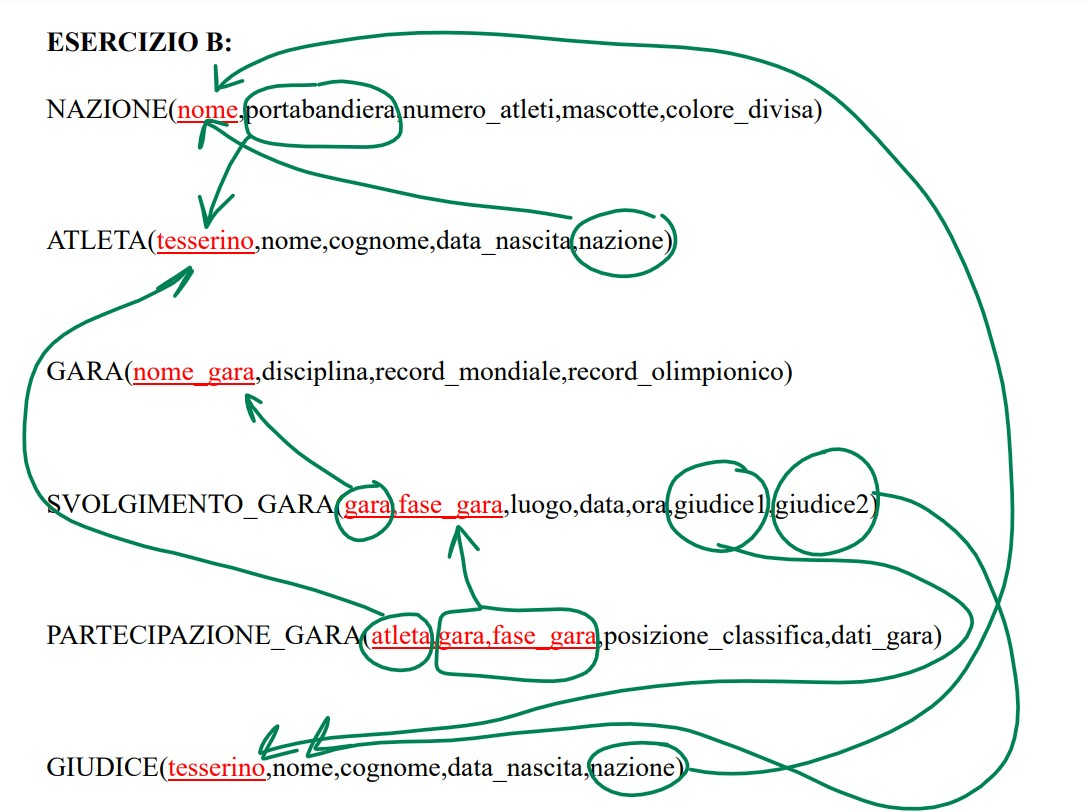
\includegraphics[width=0.675\textwidth]{chaptersLezioniSara/img/MR_fileesB.jpg}
\end{center}

\section{Es. C}
Si vuole rappresentare una base di dati relativa ai voli di una compagnia aerea. Si vuole tenere traccia dell'id del volo, del giorno della settimana, della città di partenza e di arrivo e ovviamente delle ore di partenza e arrivo. Un volo per esempio Milano-Parigi effettuato dall'aereo di tipo Airbus 300 che ha id=004 può essere svolto solo una volta durante una giornata. Per ogni tipologia di aereo si vuole tenere traccia del numero di passeggeri trasportabili, e quantità delle merci trasportabili. Ogni aeroporto è caratterizzato da una città, nazione e numero di piste. Si assuma la semplificazione che una città può avere un solo aeroporto.

\subsubsection{Identifico le relazioni}
\begin{itemize}
    \item AEROPORTO (Città, Nazione, NumPiste)
    \item AEREO (Tipo, NumPass, QuantMerci)
    \item VOLO (ID, Giorno, OraPart, OraArr, CittàPart, CittàArr, Aereo)
\end{itemize}

\subsubsection{Identifico le chiavi primarie}
\begin{itemize}
    \item AEROPORTO (\underline{Città}, Nazione, NumPiste)
    \item AEREO (\underline{Tipo}, NumPass, QuantMerci)
    \item VOLO (\underline{ID}, Giorno, OraPart, OraArr, CittàPart, CittàArr, Aereo)
\end{itemize}
\begin{center}
    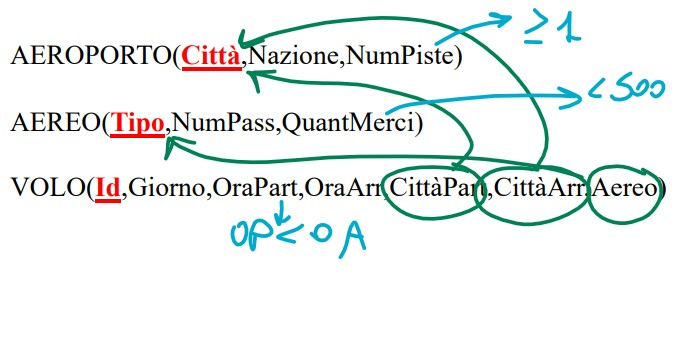
\includegraphics[width=0.675\textwidth]{chaptersLezioniSara/img/MR_fileesC.jpg}
\end{center}

\section{Es. D}
Si vuole rappresentare una base di dati relativa ai lavoratori delle aziende italiane. Per ogni lavoratore si vuole tenere traccia delle informazioni anagrafiche, delle città in cui ha abitato e lavorato e delle aziende in cui ha lavorato. Di ogni città si vuole conservare: nome, provincia e numero di abitanti. Per ogni azienda in cui le persone hanno lavorato si vuole tenere traccia del nome, P.IVA, città, numero impiegati e capitale sociale. Una azienda potrebbe aver nel tempo cambiato sede. Quindi ad esempio la Microsoft potrebbe avere avuto sede dal 1998 al 2009 a Rozzano e dal 2010 a Milano. Ogni lavoratore potrebbe aver lavorato in più aziende nel corso della sua vita.

\subsubsection{Identifico le relazioni: attributi}
\begin{itemize}
    \item PERSONA (CF, Nome, Cognome, DataNacita, CittàNascita)
    \item CITTA' (Codice, Nome, Provincia, NumAbitanti)
    \item AZIENDA (PIVA, Nome, Città, NumImpiegati, CapitaleSociale)
    \item ABITATO (Persona, Città, DataInizio, DataFine)
    \item LAVORATO (Persona, Azienda, Sede, DataInizio, DataFine)
    \item SEDE (CodiceSede, Azienda)
    \item LUOGOSEDE (CodiceSede, Città, Indirizzo, DataInizio, DataFine)
\end{itemize}
\begin{center}
    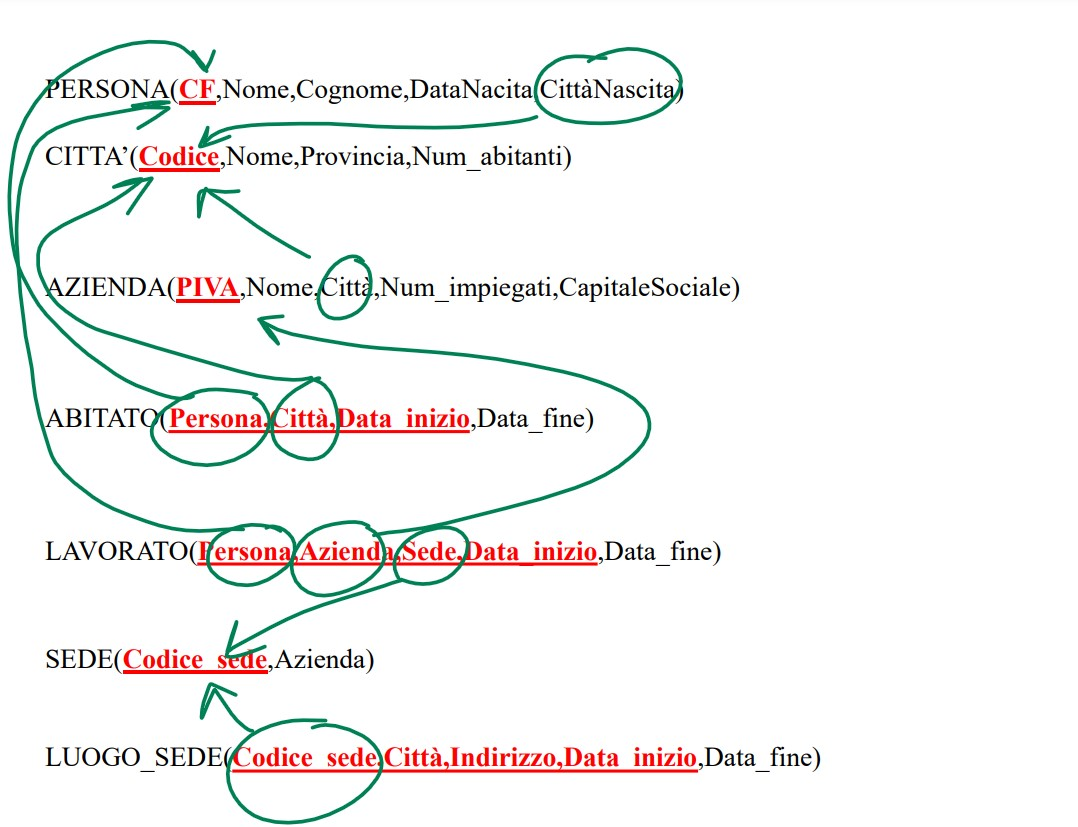
\includegraphics[width=0.675\textwidth]{chaptersLezioniSara/img/MR_fileesD.jpg}
\end{center}

\section{Es. E}
\section{Es. F}
\section{Es. G}
\chapter{Altri es. MR}
\section{Es.1 - tavolo cliente}
\subsubsection{Specifiche}
Il seguente schema relazionale riguarda un sistema di prenotazione e gestione dei tavoli di un ristorante. Il sistema in fase di prenotazione prevede una fase di registrazione in cui il cliente deve immettere i propri dati tra cui il codice fiscale, nome, cognome, e altro. Ogni tavolo ha un codice identificativo e numero di coperti massimo. Una prenotazione può riferirsi al turno pranzo o cena. Un tavolo può essere utilizzato solo una volta durante un turno. Un addetto del ristorante può servire più tavoli ma ogni tavolo è servito da un solo addetto. Ogni tavolo è dotato di un tablet attraverso cui è possibile sfogliare il menu e ordinare i pasti. Il tablet viene fornito dall'addetto al servizio al cliente ad inizio pranzo o cena. I tavoli sono disposti in diverse sale separate che possono essere 'normali' o sale in cui si proiettano eventi sportivi e concerti.

\subsubsection{Relazioni}
TABLET (codice, marca, modello, dataAcquisto, scadenzaGaranzia)
\\TAVOLO (codice, numeroCoperti, sala)
\\CLIENTE (codiceFiscale, nome, cognome, indirizzo, cap, citta, numTel, email)
\\GESTIONETAVOLO (codiceTavolo, cliente, data, turno, addettoRistorante, tablet)
\\PERSONALERISTORANTE (codiceFiscale, nome, cognome, stipendio, annoNascita, annoAssunzione)
\\SALA (codice, tipologia)

\subsubsection{Chiavi primarie}
TABLET (\underline{codice}, marca, modello, dataAcquisto, scadenzaGaranzia)
\\TAVOLO (\underline{codice}, numeroCoperti,sala)
\\CLIENTE (\underline{codiceFiscale}, nome, cognome, indirizzo, cap, citta, numTel, \underline{email})
\\GESTIONETAVOLO (\underline{codiceTavolo}, cliente, \underline{data}, \underline{turno}, addettoRistorante, tablet)
\\PERSONALERISTORANTE (\underline{codiceFiscale}, nome, cognome, stipendio, annoNascita, annoAssunzione)
\\SALA (\underline{codice}, tipologia)

\subsubsection{Chiavi esterne}
\begin{center}
    \includegraphics[width=0.675\textwidth]{chaptersLezioniSara/img/MR_altrofile_es1.jpg}
\end{center}

\subsubsection{Vincoli di tupla}
data.acquisto < scadenza + 2
\\anno-nascita $\leq$ anno-assunzione + 18
\\CAP = seq numeri interi L = 5
\\numero-coperti > 0

\section{Es.2 - gestione magazzino}
\subsubsection{Specifiche}
Il seguente schema relazionale riguarda un sistema per la gestione di una palestra. In palestra possono entrare solo gli iscritti con abbonamento in corso di validità. All'entrata gli iscritti utilizzano un badge che permette di aprire il tornello di entrata solo se l'abbonamento è in corso di validità. Gli abbonamenti possono essere di diversa tipologia: mezza giornata, giornata piena ecc.. La palestra è composta da sale ognuna destinata ad una tipologia di attività: attrezzi, corpo libero ecc. In una data sala viene svolta una specifica attività e opera un solo addetto. Nelle sale possono esserci degli attrezzi. Dalla palestra vengono offerte gratuitamente (incluso nell'abbonamento) delle lezioni di gruppo come «lezione di aerobica», «zumba» ecc. che sono svolte in un dato giorno e ora della settimana in una data sala sempre dallo stesso addetto.

\subsubsection{Relazioni}
ATTREZZATURA (codice, marca, modello, dataAcquisto, scadenzaGaranzia, sala)
\\LEZIONE (codiceLezione, nome, giorno, ora, sala, addetto)
\\ISCRITTO (codiceFiscale, nome, cognome, indirizzo, cap, citta, numTel, email)
\\ABBONAMENTO(iscritto, dataInizio, dataFine, tipologia)
\\ADDETTO (codiceFiscale, nome, cognome, stipendio, annoNascita, annoAssunzione)
\\SALA (codice, tipologiaAttività, addetto)

\subsubsection{Chiavi primarie}
ATTREZZATURA (codice, marca, modello, dataAcquisto, scadenzaGaranzia, sala)
\\LEZIONE (codiceLezione, nome, giorno, ora, sala, addetto)
\\ISCRITTO (codiceFiscale, nome, cognome, indirizzo, cap, citta, numTel, email)
\\ABBONAMENTO(iscritto, dataInizio, dataFine, tipologia)
\\ADDETTO (codiceFiscale, nome, cognome, stipendio, annoNascita, annoAssunzione)
\\SALA (codice, tipologiaAttività, addetto)

\subsubsection{Vincoli di tupla}
data acquisto < scadenza garanzia
\\data inizio < data fine
\\anno nascita $\leq$ anno assunzione 

\section{Es.3 - libreria}
\subsubsection{Specifiche}
Lo schema seguente rappresenta una base di dati impiegata in una catena di librerie distribuite su tutto il territorio nazionale. In particolare, oltre ai dati sulle singole librerie, sono archiviati i dati del personale e dei libri in vendita. Si osservi che possono esistere diverse versioni dello stesso libro (autore e titolo), edite da case editrici diverse. Infine, attraverso la relazione Catalogo è possibile conoscere in quali librerie una determinata versione di un libro sia disponibile per essere venduta, il numero di copie a disposizione, ed il costo. 

\subsubsection{Relazioni}
LIBRERIA(idLibreria, indirizzo, città, oraApertura, oraChiusura, turnoChiusura)
\\PERSONALE(idPersona, cognome, nome, idLibreria, reparto, turno)
\\CATALOGO(idLibro, idLibreria, reparto, numerocopie, costo)
\\LIBRO(idLibro, titolo, autori, casaEditrice, annoPubblicazione)

\subsubsection{Chiavi primarie}
LIBRERIA(\underline{idLibreria}, indirizzo, città, oraApertura, oraChiusura, turnoChiusura)
\\PERSONALE(\underline{idPersona}, cognome, nome, idLibreria, reparto, turno)
\\CATALOGO(\underline{idLibro}, \underline{idLibreria}, reparto, numerocopie, costo)
\\LIBRO(\underline{idLibro}, titolo, autori, casaEditrice, annoPubblicazione)

Chiavi alternative:
\\"indirizzo" e "città" per Libreria.

Possibile superchiave:
\\tutta la tupla di una qualsiasi relzione, es la riga di Libro.

\subsubsection{Vincoli di ennupla}
orario apertura < orario chiusura

\subsubsection{Vincoli di dominio}
costo > 0
\\numerocopie $\geq$ 0
\\turnoChiusura $\in$ {lunedi, martedi, mercoledi, giovedi, venerdi, sabato, domenica}
\chapter{Algebra Relazionale}
\section{Dai modelli ai linguaggi}
I modelli concettuali e logici permettono di descrivere informazioni, ma non sono direttamente interpretabili da un elaboratore. Dai modelli dobbiamo passare ai linguaggi, dotati di: 
\begin{description}
    \item[sintassi], che definisce le frasi corrette del linguaggio 
    \item[semantica], che definisce le operazioni effettuate quando vengono eseguite gli operatori (o istruzioni o comandi) del linguaggio
\end{description}

\subsection{Linguaggi per Basi di Dati}
\begin{center}
    \includegraphics[width=0.675\textwidth]{chaptersLezioniSara/img/AR_linguaggi1.jpg}
\end{center}

\subsection{Tipi di linguaggi}
\subsubsection{Procedurali}
Specificano le modalità di generazione del risultato ("come").
\subsubsection{Dichiarativi}
Specificano le proprietà del risultato ("che cosa").

\subsection{Linguaggi per Basi di Dati Relazionali} 
\begin{description}
    \item[Algebra relazionale]: procedurale
    \item[Calcolo relazionale]: dichiarativo 
    \item[SQL]: (parzialmente) dichiarativo 
    \item[QBE](Query by Example): dichiarativo
\end{description}

\section{AR vs SQL}
Capire l'algebra è la chiave per la comprensione dell'SQL. L'algebra relazionale è un linguaggio procedurale, mentre SQL è un linguaggio dichiarativo.
\begin{center}
    \includegraphics[width=0.675\textwidth]{chaptersLezioniSara/img/AR_linguaggi2.jpg}
\end{center}

\subsubsection{AR}
Linguaggio prettamente formale che forma la base per linguaggi 'reali'.
\\Linguaggio procedurale: si specifica l'algoritmo con cui ottenere il risultato.
\\Istruzioni equivalenti possono differire in termini di efficienza.
\\Relazioni intese in senso matematico => Insiemi di tuple, definite su attributi.
\\Negli insiemi non ci possono essere elementi uguali.

\subsubsection{SQL}
Linguaggio più usato per basi di dati relazionali.
\\Linguaggio (parzialmente) dichiarativo: si specifica il risultato da ottenere senza preoccuparsi di specificare l'algoritmo.
\\Istruzioni equivalenti differiscono solo per leggibilità.
\\Relazioni intese come tabelle.
\\Possono esserci righe uguali.

\section{Algebra Relazionale}
Insieme di operatori:
\begin{itemize}
    \item su relazioni
    \item che producono relazioni
    \item e possono essere composti tra loro a formare nuove interrogazioni
\end{itemize}
\subsubsection{Operatori AR}
\begin{center}
    \includegraphics[width=0.675\textwidth]{chaptersLezioniSara/img/AR_operatori1}
\end{center}
\subsubsection{Operatori che vedremo in questa lezione}
\begin{center}
    \includegraphics[width=0.675\textwidth]{chaptersLezioniSara/img/AR_operatori2}
\end{center}

\section{Operatori insiemistici}
\subsection{Le relazioni sono insiemi}
In matematica una relazione è un sottoinsieme del prodotto cartesiano di due o più insiemi
\\Il prodotto cartesiano degli insiemi D1, D2, … DN indicato come D1 x D2 x ... x Dn è l'insieme di tutte le n-uple ordinate (d1,d2,...,dn) tali che d1 ∈ D1, d2 ∈ D2, ... , dn ∈ Dn
% 5 slides di immagini
Una relazione è un insieme quindi:
\begin{itemize}
    \item non c'è ordinamento tra le diverse tuple
    \item le tuple sono dis6nte (non ce ne possono essere due uguali)
    \item ciascuna tupla è al suo interno ordinata: l'i-esimo valore proviene dall'i-esimo dominio
\end{itemize}
NB: una tabella è una relazione SOLO se non ci sono righe uguali.
\subsection{L'operatore Intersezione}
\subsection{L'operatore Differenza}

\section{Limiti degli operatori insiemistici}
\subsection{L'operatore di ridenominazione}





% www.wooclap.com/SCSYHF
\section{Select}
\section{Join}
\chapter{Progettazione Logica}
Ci vorrà ancora un po' per i risultati, ma non manca tanto.\\
La seconda parte, il secondo compitino, prevede 
\begin{itemize}
    \item la progettazione logica
    \item il secondo esercizio
    \item il terzo esercizio
\end{itemize}
Secondo il prof. Napoletano, la progettazione logica è abbastanza equiparabile al Modello Relazionale.\\
Viene presentato uno schema ER generico con proprietà ben determinate, senza una specifica, di cui bisogna identificare determinate regole di ristrutturazione prima di tradurre il modello destrutturato in un elenco di tabelle.
\section{Progettazione Logica}
\begin{center}
    \includegraphics[scale=0.675]{chaptersLezioniSara/img/PLog_intro1.jpg}
\end{center}
Come già precedentemente detto, non vedremo a lezione la progettazione fisica (è prevista a laboratorio però).\\
Richiede di scegliere il modello dei dati modello relazionale.
\subsubsection{Obiettivo}
Definizione di uno schema logico relazionale corrispondente allo schema ER di partenza.
\subsubsection{Aspetti importanti}
Semplificazione dello schema per renderlo rappresentabile mediante il modello relazionale ottimizzazione per aumentare l'efficienza delle interrogazioni.

\subsection{Obiettivo}
"Tradurre" lo schema concettuale in uno schema logico che rappresenti gli stessi dati in maniera corretta ed efficiente.

\subsubsection{Ingresso:}
\begin{itemize}
    \item schema concettuale
    \item informazioni sul carico applicativo
    \item modello logico
\end{itemize}
\subsubsection{Uscita:}
\begin{itemize}
    \item schema logico
    \item documentazione associata
\end{itemize}
\begin{center}
    \includegraphics[scale=0.675]{chaptersLezioniSara/img/PLog_intro2.jpg}
\end{center}
Non si tratta di una pura e semplice traduzione
\begin{itemize}
    \item alcuni aspetti non sono direttamente rappresentabili
    \item è inoltre necessario considerare le prestazioni
\end{itemize}
\begin{center}
    \includegraphics[scale=0.675]{chaptersLezioniSara/img/PLog_intro3.jpg}
\end{center}

\subsection{Ristrutturazione schema E-R}
Eliminazione dallo schema E/R di tutti i costrutti che non possono essere direttamente rappresentati nel modello logico target (relazionale nel nostro caso):
\begin{itemize}
    \item Eliminazione degli attributi multivalore
    \item Eliminazione delle generalizzazioni
\end{itemize}
Inoltre:
\begin{itemize}
    \item Partizionamento/accorpamento di entità e associazioni
    \item Scelta degli identificatori primari
    \item Analisi ridondanze (non dovrebbero esserci, \dots)
\end{itemize}
\begin{center}
    \includegraphics[scale=0.675]{chaptersLezioniSara/img/PLog_intro4.jpg}
\end{center}
\subsubsection{Motivazioni:}
\begin{itemize}
    \item semplificare la traduzione
    \item "ottimizzare" le prestazioni
\end{itemize}
\subsubsection{Osservazione:}
\begin{itemize}
    \item uno schema E-R ristrutturato non è (più) uno schema concettuale nel senso stretto del termine
\end{itemize}
\textbf{Per ottimizzare il risultato abbiamo bisogno di analizzare le prestazioni a questo livello.}\\
Ma:
\begin{itemize}
    \item le prestazioni non sono valutabili con precisione su uno schema concettuale:
    \item Dipendono dalle caratteristiche del DBMS
    \item bisogna conoscere il volume dei dati e le caratteristiche delle operazioni
\end{itemize}

\subsection{Carico applicativo}
Consideriamo degli "indicatori" dei parametri che regolano le prestazioni:
\begin{itemize}
    \item \textit{tempo di esecuzione} delle operazioni di principale interesse: numero di istanze (di entità e relazioni) mediamente accedute durante l'esecuzione dell'operazione \textit{(accessi)}
    \item \textit{spazio di memoria} necessario per memorizzare i dati di interesse
\end{itemize}
Per valutare questi parametri bisogna conoscere (oltre allo schema):
\subsubsection{volume dei dati:}
\begin{itemize}
    \item numero di istanze previste di entità e relazioni
    \item dimensione di ciascun attributo
\end{itemize}
\subsubsection{caratteristiche delle operazioni:}
\begin{itemize}
    \item tipo: interattiva o batch
    \item frequenza: numero medio di esecuzioni in un certo periodo
    \item dati coinvolti
\end{itemize}
Si noti che la valutazione sarà necessariamente approssimata, in quanto le prestazioni effettive della base di dati dipendono anche da parametri fisici, difficilmente prevedibili in questa fase (DBMS utilizzato, indici, \dots).

\subsection{Schema di operazione}
Lo schema di operazione descrive i dati coinvolti in un'operazione.\\
Corrisponde al frammento dello schema ER interessato all'operazione sul quale viene disegnato il cammino logico per accedere alle informazioni di interesse.\\
\begin{center}
    \includegraphics[scale=0.675]{chaptersLezioniSara/img/PLog_intro5.jpg}
\end{center}
Ma perché questo schema è importante? Per le operazioni che devo affrontare che possono essere molto ripetitive.

\subsection{Esempio 1}
\begin{center}
    \includegraphics[scale=0.675]{chaptersLezioniSara/img/PLog_intro_es1.jpg}
\end{center}
Per calcolare il numero di accessi a Turno e Autobus occorre conoscere il numero medio di Turni per Autista (MT).

\subsection{Tavola degli accessi}
Con lo schema di operazione si può fare una stima del costo di un'operazione contando il numero di accessi alle istanze di entità e relazioni.\\
Il risultato può essere riassunto in una \textbf{tavola degli accessi}.
\begin{center}
    \includegraphics[scale=0.675]{chaptersLezioniSara/img/PLog_tavolaAccessi1.jpg}
\end{center}
Il tipo distingue gli accessi in scrittura (S) e in lettura (L).\\
Le operazioni di scrittura sono in genere più onerose (esecuzione in modo esclusivo, aggiornamento degli indici).

\subsection{Esempio 1}
\begin{center}
    \includegraphics[scale=0.675]{chaptersLezioniSara/img/PLog_tavolaAccessi_es1.jpg}
\end{center}
\subsection{Esempio 2}
\begin{center}
    \includegraphics[scale=0.675]{chaptersLezioniSara/img/PLog_tavolaAccessi_es2.jpg}
\end{center}

\subsection{Esempio di valutazione di costo}
Schema E-R:
\begin{center}
    \includegraphics[scale=0.675]{chaptersLezioniSara/img/PLog_tavolaAccessi_es3a.jpg}
\end{center}
\begin{description}
    \item[Operazione:] trova tutti i dati di un impiegato, del dipartimento nel quale lavora e dei progetti ai quali partecipa.
\end{description}
Si costruisce una \textbf{tavola degli accessi} basata su uno \textbf{schema di navigazione}.
\begin{description}
    \item[Schema di navigazione:] parte dello schema E/R interessata dall'operazione, estesa con delle frecce che indicano in che modo l'operazione "naviga" i dati.
\end{description}
\begin{center}
    \includegraphics[scale=0.675]{chaptersLezioniSara/img/PLog_tavolaAccessi_es3b.jpg}
\end{center}
Tavola dei volumi:
\begin{center}
    \includegraphics[scale=0.675]{chaptersLezioniSara/img/PLog_tavolaAccessi_es3c.jpg}
\end{center}
Specifica il numero stimato di istanze per ogni entità (E) e associazione (R) dello schema. I valori sono necessariamente approssimati, ma indicativi. Il numero (medio) di partecipazioni di una istanza di entità alle istanze di relazione (dipende dalla cardinalità delle relazioni).

\subsection{Attività della ristrutturazione}
Analisi delle ridondanze.\\
Eliminazione delle generalizzazioni/gerarchie.\\
Partizionamento/accorpamento di entità e relationship.\\
Eliminazione attributi multivalore.\\
Scelta degli identificatori primari

\subsection{Analisi delle ridondanze}
Una ridondanza in uno schema E-R è una informazione significativa ma derivabile da altre.\\
In questa fase si decide se eliminare le ridondanze eventualmente presenti o mantenerle.

\subsection{Ridondanze}
Vantaggi
\begin{itemize}
    \item semplificazione delle interrogazioni
\end{itemize}
Svantaggi
\begin{itemize}
    \item appesantimento degli aggiornamenti
    \item maggiore occupazione di spazio
\end{itemize}

\subsection{Forme di ridondanza in uno schema E-R}
Attributi derivabili:
\begin{itemize}
    \item da altri attributi della stessa entità (o relazione)
    \item da attributi di altre entità (o relazioni)
\end{itemize}
Associazioni derivabili dalla composizione di altre relazioni in presenza di cicli.

\subsubsection{Attributi derivabili}
Il valore di un attributo si calcola sulla base delle altre proprietà.
\begin{center}
    \includegraphics[scale=0.675]{chaptersLezioniSara/img/PLog_ridondanze1.jpg}
\end{center}

\subsubsection{Attributi derivabili da un'altra entità}
Attributo calcolato sulla base degli attributi di un'altra entità.
\begin{center}
    \includegraphics[scale=0.675]{chaptersLezioniSara/img/PLog_ridondanze2.jpg}
\end{center}
\begin{center}
    \includegraphics[scale=0.675]{chaptersLezioniSara/img/PLog_ridondanze3.jpg}
\end{center}
L'attributo MediaVoti è ridondante.\\
• utile per velocizzare le interrogazioni relative al calcolo della media dei voti degli studenti.\\
• se conservato, occorre integrare lo schema relazionale con l'indicazione di ridondanza dell'attributo.\\

Vabbeh facciamo che ascolto e basta, mi sono persa.\\
\`E arrivato alla slide 49/142.








\end{document}
